\documentclass[12pt]{gatech-thesis}
\usepackage{amsmath,amssymb,latexsym,float,epsfig,subfigure,graphicx,listings,hyperref}

\title{Integrating Reinforcement Learning into a Programming Language}

\author{Christopher Simpkins}
\department{School of Interactive Computing}


\principaladvisor{Professor Charles L. Isbell, Jr.}[School of
  Interactive Computing]
\committeechair{}
\firstreader{Dr. Douglas Bodner}[Tennenbaum Institute]
\secondreader{Professor Mark Riedl}[School of Interactive Computing]
\thirdreader{Dr. Spencer Rugaber}[School of Computer Science]
\fourthreader{Professor Andrea Thomaz}[School of Interactive Computing]


\degree{Doctor of Philosophy}


%% Set \listmajortrue below, then uncomment and set this for
%% interdisciplinary PhD programs so that the title page says
%% ``[degree] in [major]'' and puts the department at the bottom of
%% the page, rather than saying ``[degree] in the [department]''

%% \major{Algorithms, Combinatorics, and Optimization}
\major{Computer Science}

\copyrightyear{2016}
\submitdate{15 December 2016}

%% The date the last committee member signs the thesis form. Printed
%% on the approval page.
\approveddate{TBD}


\bibfiles{references}

%% The following are the defaults
%%    \titlepagetrue
%%    \signaturepagetrue
%%    \copyrightfalse
%%    \figurespagetrue
%%    \tablespagetrue
%%    \contentspagetrue
%%    \dedicationheadingfalse
%%    \bibpagetrue
%%    \thesisproposalfalse
%%    \strictmarginstrue
%%    \dissertationfalse
%%    \listmajorfalse
%%    \multivolumefalse

\listmajortrue
\dissertationtrue

%% \thesisproposaltrue

\includeonly{introduction}
\includeonly{rl}
\includeonly{arbiq}

\begin{document}
\nocite{*}
\bibliographystyle{gatech-thesis}
%%
\begin{preliminary}
\begin{dedication}
\null\vfil
{\large
\begin{center}
To my children,\\\vspace{12pt}
Isaac and Meredith,\\\vspace{12pt}
who motivated my decision to give up flying and enter academia.
\end{center}}
\vfil\null
\end{dedication}
%\begin{preface}

%\end{preface}
%\begin{acknowledgements}

%\end{acknowledgements}
% print table of contents, figures and tables here.
\contents
% if you need a "List of Symbols or Abbreviations" look into
% gatech-thesis-gloss.sty.

\begin{summary}
\vspace{-1in}

Improving the composability of modules in modular reinforcement learning and integrating modular reinforcement learning into a programming language supports reuse in adaptive agent software engineering.  This thesis claims that (1) modular reinforcement learning can be extended to support composability in modular reinforcement learning agents by uncoupling the reward scales of the modules that comprise the agents, and (2) integrating modular reinforcement learning into a programming language supports adaptive agent programming by reducing the effort required to write agent programs and adapt them to new domains.

Composability, an essential property of modularity in software engineering, allows components to be reused in the construction of new systems.  In the case of a modular reinforcement learning agent composability means being able to reuse behavior modules in new agents without modifying the modules.  The current state of the art in modular reinforcement learning supports decomposition but not composition, or module reuse.  This dissertation contributes a reformulation of modular reinforcement learning -- command arbitration -- that supports composition by uncoupling the reward scales of the modules that comprise a modular reinforcement learning agent, and a new command arbitration algorithm for modular reinforcement learning.

An excellent way to support software engineering is with practical, usable programming languages.  The second major contribution of this dissertation is an domain-specific language and framework embedded in the Scala programming language that integrates modular reinforcement learning.  We show how this integration is useful to software engineers writing practical adaptive agent software by applying AFABL to representative agent programming tasks and measuring the benefit of integrated modular reinforcement learning compared to traditional programming.  This application to practical software engineering problems distinguishes AFABL from previous work in integrating RL into programming languages such as ALisp.

\end{summary}

\end{preliminary}

\cleardoublepage

\chapter{Introduction}

\begin{quote}
If you don't know where you are going, any road will take you there.\\
  -- Lewis Carroll, paraphrased from Alice's Adventures in Wonderland
\end{quote}


This chapter sets the stage for the work presented in this dissertation, an overview of its contributions, and concludes with a road-map of the following chapters.


\section{The Dream of AI}

Artificial intelligence was one of the first grand promises of computing. Almost as soon as the field of computer science was born the pioneers of AI were promising machines that could think and act as well as humans within the ``visible future'' (Herbert Simon, quoted in 1958). Early research in AI focused on machines that could ``think'' like humans and employed symbolic computation to create constraint solvers, planners, and exert systems that used truth maintenance systems to maintain sets of facts and inference rules that produced new knowledge. We had computer programs that solved algebra equations, found paths, played games, and diagnosed illnesses based on user-reported symptoms. Symbolic, or knowledge-based AI hit a bottleneck in the late 1980s -- commonly called the knowledge acquisition bottleneck -- and the early promise of developing systems that {\it replaced} humans faded. But AI in general did not fade. AI reinvented itself. Instead of creating systems of rules and inference engines based on encoded knowledge, modern AI applies well-developed models from mathematics and engineering -- vector space models for text retrieval, hidden Markov models for speech recognition, neural networks (though originally invented within AI but then abandoned and developed by electrical engineers) for image recognition -- to problems traditionally considered part of AI. In modern AI the emphasis is on rationality -- achieving optimal results without trying to explicitly mimic human cognition -- and in developing systems that assist humans in some way. In modern AI every approach must have a performance measure that is being optimized -- speech phoneme recognition rate, generalization error in image classifiers, etc. -- and AI algorithms are not accepted if they do not either define a new category rigorously, or rigorously compare their performance to existing algorithms using accepted performance criteria. Most AI algorithms today are concerned with focused problems and find application in software that assists humans, such as helping humans find the right books to buy using collaborative filtering or finding photos of their babies using facial image recognition.  Reinforcement learning is notable for applying modern AI approaches to the age old intelligent agent problem: given the state of the world and all the actions an agent {\it could} take, which action {\it should} the agent take\added[id=v3]{, that is, which action results in the agent accumulating the greatest long-term reward}.

One can think of reinforcement learning (RL) as a machine learning approach to planning, that is, a way of finding a sequence of actions that achieves a goal.  The RL problem formulation is this: an agent's world is described by a set of states, the agent can execute an action from a prescribed set of actions in each state, and the agent is rewarded to greater or lesser degrees for each state-changing action it executes. The performance measure being optimized by reinforcement learning algorithms is long-term expected reward. So a reinforcement learning agent learns delayed gratification. For example, eating cake now provides high immediate reward but low long-term reward. A reinforcement learning agent learns to choose salad over cake (unless the agent is Ron Swanson). For the software engineer who would like to employ reinforcement learning without becoming an expert the most important thing to understand is that the world of an agent can be modeled in terms of states, actions, and one-step rewards. Our work shows that if you can specify the states, actions, and rewards for an agent our algorithms can work behind the scenes to develop a control policy.

\section{The Challenges of Software Engineering}

Software engineering has struggled to keep pace with the growing size and complexity of the systems being demanded by users. Over time the field of software engineering, both in academia and industry, has developed a well-defined set of practices and design guidelines that result in software systems that are maintainable, reliable and extensible. Programming languages have been a primary means by which research in software engineering and formal computer science has been brought to bear for the working programmer. From structured programming to object-oriented programming to powerful modern type systems, important advances in computing research have real impact when they are incorporated as features in practical programming languages. In the same way that, say, formal methods are used by the modern programmer in the form of static type systems without requiring the programmer to know much about formal methods, AFABL's goal is to allow the programmer to use reinforcement learning without knowing much about reinforcement learning algorithms.

\section{The Promise of Adaptive Partial Programming}

Our work in integrating reinforcement learning into a programming language is based on the idea of partial programming developed by researchers in hierarchical reinforcement learning. Partial programming is a framework for programming in which a programmer or designer specifies the structure of certain parts of the system while leaving other portions unspecified, such that a learning system can learn how to perform them. Hierarchical reinforcement learning defines closed-loop policies that group action sequences into logical units -- subroutines -- that achieve intermediate goals. For example, if the ultimate goal of an agent is to leave a building by exiting a room and walking down an hall, and the agent's primitive actions are MOVE-FORWARD, MOVE-LEFT, TURN-RIGHT and so-on, then one of the agent's subroutines might be FIND-DOOR, which achieves the intermediate goal of exiting the room. Partial programming system allows the agent designer to specify intermediate goals, write code to achieve certain goals, and let reinforcement learning algorithms learn how to achieve the others.

Hierarchical reinforcement learning decomposes the reinforcement learning problem temporally, that is, it breaks action sequences into subsequences. Another kind of adaptive programming -- known as modular reinforcement learning (MRL) -- is based on concurrent problem decomposition in which an agent may take only one action at a time but must pursue several goals simultaneously. MRL is especially well suited to continuing problems in which an agent is never ``done'' pursuing certain goals. For example, for the entire time it is operating a self-driving car will need to avoid other vehicles, optimize speeds for road conditions subject to speed limits, maximize fuel economy, minimize travel time, and so on.

MRL is a developing field with few algorithms and a small number of programming systems attempting to make MRL usable for working programmers. Currently available algorithms for MRL and programming systems based on them suffer from a reward coupling problem: modules used within the same agent must be authored together to ensure reward scales are comparable. This reward coupling is an impediment to module reuse in practical software engineering because an existing module can not simply be reused in a new context without re-engineering its reward function. Our work solves this problem with a reformulation of MRL and an algorithm that makes module reuse possible, and integrates this new kind of MRL in a practical programming language.


\section{Contributions}

The work presented in this dissertation marries artificial intelligence and software engineering in a way that advances both fields. The needs of practical software engineering for reuse and composability inspires a new AI algorithm for modular reinforcement learning. Integrating this new formulation of modular reinforcement learning and associated algorithms into a programming language enables a new kind of software engineering: modular adaptive agent programming. In particular, this work makes the following contributions:

\begin{itemize}
\item We explain a problem with the current state of the art in modular reinforcement learning, namely, that performance degrades if modules have differing, incomparable reward scales. \added[id=v3]{While there may be other incompatibility problems, such as synchronization and impedence mismatch, we focus on reward incomparability because our goal is to enable independently authored modules.}
\item We empirically demonstrate the performance degradation of modular reinforcement learning agents whose modules have incomparable reward scales.
\item We present an analysis of the shortcoming of current approaches to modular reinforcement learning based on Arrow's Impossibility Theorem for social choice in order to frame our solution.
\item We reformulate the modular reinforcement learning problem as one of {\it command arbitration} instead of merging MDPs or Q-functions.
\item We present a command arbitration algorithm -- Arbi-Q -- that uses our theoretically grounded reformulation of modular reinforcement learning.
\item We empirically demonstrate that modular reinforcement learning agents using Arbi-Q exhibit no performance degradation when modules have incomparable reward scales.
\item We present a Scala-embedded domain-specific language -- AFABL -- that integrates modular reinforcement learning and our Arbi-Q command arbitration algorithm.
\item We demonstrate and quantify the value of integrating modular reinforcement learning into a programming language to practical software engineering in a programmer study applying AFABL in a synthetic agent programming domain.
\item We apply AFABL to a practical problem in psychology-based human agent modeling to demonstrate AFABL's practical potential.
\end{itemize}

\section{Outline}

In the following chapters we present the two major contributions of this dissertation: command arbitration for modular reinforcement learning and a practical agent programming language that integrates modular reinforcement learning: AFABL. For both major contributions there is a chapter providing the necessary background, then a chapter presenting our contributions. Related work is provided in each chapter where it is most relevant rather than gathered in a single place.

Chapter \ref{ch:rl} provides background information in modular reinforcement learning and existing approaches to modular reinforcement learning.

Chapter \ref{ch:arbiq} presents an empirical demonstration of the performance degradation of modular reinforcement learning agents whose modules have incomparable reward scales. Arrow's Impossibility Theorem for social choice provides an explanation for the failure of existing approaches to modular reinforcement learning and a framework for our solution. We present our solution, the Arbi-Q command arbitration algorithm, and empirically demonstrate that it does not exhibit the same performance degradation as existing approaches to modular reinforcement learning.

Chapter \ref{ch:se} provides background information on software engineering that motivates the use of modular reinforcement learning in building practical software systems, and the integration of modular reinforcement learning into a programming language.

Chapter \ref{ch:afabl} presents a programming language, AFABL, which integrates modular reinforcement learning. AFABL, a domain-specific language embedded in the Scala language, allows programmers to write adaptive software agents in a declarative style using elements of modular reinforcement learning: modules with states, actions, and rewards. We present the results of a programmer study that shows the value of integrating reinforcement learning into a programming language: AFABL agents are less complex, easier to write, and easier to adapt to changes in the environment.

Chapter \ref{ch:applications} presents a practical application of AFABL that further demonstrates the usefulness of integrating modular reinforcement learning into a programming language.

Chapter \ref{ch:conclusion} concludes the dissertation by reviewing how the central theses of this dissertation were confirmed and the present work's context, limitations, and consequences and discuss directions for future work.


\chapter{Background in Reinforcement Learning}\label{ch:rl}

The field of reinformcement learning is large and growing. In this chapter we provide the background in reinforcement learning and modular reinformcenet learning necessary to understand our work and place it in context.

\section{Reinforcement Learning}

One can think of reinforcement learning (RL) \cite{sutton1998reinforcement,kaelbling1996reinforcement} as a machine learning approach to planning, that is, as a way of finding a sequence of actions that achieves a goal. In RL, problems of decision-making by agents interacting with uncertain environments are usually modeled as Markov decision processes (MDPs). In the MDP framework, at each time step the agent senses the state of the environment and executes an action from the set of actions available to it in that state. The agent's action (and perhaps other uncontrolled external events) cause a stochastic change in the state of the environment. The agent receives a (possibly zero) scalar reward from the environment. The agent's goal is to find a {\it policy}; that is, to choose actions so as to maximize the expected sum of rewards over some time horizon. An optimal policy is a mapping from states to actions that maximizes the long-term expected reward.  In short, a policy defines which action an agent should take in a given state to maximize its chances of reaching a goal.

\subsection{Markov Decision Processes}

The basic Markov decision process is a 3-tuple,

\begin{equation}
(S, A, T(s, a, s'))
\end{equation}

where

\begin{itemize}
\item $S$ is a set of states,
\item $A$ is a set of actions, and
\item $T(s, a, s')$ is a transition function which gives the probably that executing action $a$ in state $s$ will result in $s'$.
\end{itemize}

Most definitions of MDPS include a reward function, $R(s, a, s')$ which specifies the reward that the world provides to an agent for taking action $a$ in state $s$ and arriving in state $s'$, or equivalently simply a reward for arriving in state $s$, $R(s)$. Some definitions of MDPS include an initialization function, $I(s)$, which specifies the probablity the the agent will start in some state $s \in S$, others specify a particular state from $S$ as the start state.

We prefer to think of the basic 3-tuple MDP as representing the states and state transition dynamics of a world, and an agent solving a Markov Decision {\it Problem} which adds the reward function, initialization function, and discount factor. We believe this distinction between Markov Decision {\it Processes} and Markov Decision {\it Problems} leads to a more natural expression of worlds and agents for programmer who are not familiar with the underlyiung theory of reinforcement learning. For example, most people would not include a single universal reward function as part of the ``world'' because different agents may value different states differently. Similarly, different agents may have a shorter or longer term view of decision optimality and thus different discount factors. Separating the world dynamics from the agent's use of the world dynamics doesn't change the reinformcement learning algorithms, but as we will see in Chapter \ref{ch:afabl}, separating worlds from agents is useful in practical programming.

The solution to a Markov Decision Problem is a policy, denoted $\pi$, which is a mapping from states to actions. The policy says, for any state, what is the best action to take in order to maximaze the agent's long term reward.

\subsection{Long Term Reward}

Acting optimally in the world means maximizing your long term reward. In the MDP setting there are many ways to compute long term reward depending on whether you consider rewards gained during a finite or infinite time horizon, can depend on there being a terminal state the agent is guaranteed to reach, or whether the agent's task is episodic or continuing. The most commonly used formulation of long term which is geometrically discounted rewards over an infinite time horizon, which works for episodic taks, continuing tasks, and results in stationary policies, that is, policies that depend only on the current state.

\begin{equation}
R_t = \sum_{k=0}^{\infty} \gamma^k r_{t+k+1}
\end{equation}

We use this conception of long term reward to calcluate the values of states.


\subsection{Value Functions}

A value function assigns a number to each state indicating how good is it for an agent to be in that state. If you know the values of all the possible next states of your current state, then the action you should take is the action most likey to get you into the next state having the highest value.

The value of a state (or state, action pair) under a particular policy $\pi$ is the expected long term reward an agent would get starting from state $s$ if it followed $\pi$. The value is computed from the rewards and state transition dynamics of a world as follows:

\begin{equation}
V^\pi(s) = E \left [ \sum_{t=0}^{\infty} \gamma^t R(s_t) \right ]
\end{equation}

State value functions form the basis of dynamic programming approaches to solving MPDs. The reinforcement learning algorithms we discuss in Section \ref{sec:rl} use action value functions, which assign values directly to the actions available in a given state.

\subsection{Optimal Policies}

Since some states have higher values than others, and some actions have higher probabilities of causing transitions to higher-valued successor states, there is an optimal action in each state, namely, the action most likely to cause a transition to the highest-valued successor state. The optimal actions in each state is the optimal policy:

\begin{equation}
\pi^*(s) = \argmax_{a \in A} \sum_{s'} T(s, a, s') V(s')
\end{equation}

There may be many optimal policies for a given MDP, but without loss of generality we usually simply say ``the optimal policy.''

\subsection{Solving MDPs with Dynamic Programming}

If you have the MDP -- you know the transition function and reward function -- you can solve for the value of each state using value iteration, from which the optimal policy is derived, or find the policy directly using policy iteration. Although a practical reinforcement learning agent usually doesn't have the full MDP model, the theory of dynamic programming is useful in understanding reinforcement learning algorithms.

\subsubsection{Value Iteration}

Previously we defined the value of a state under a particular policy. If we assume the optimal policy, we can define the maximum value of a state in terms of optimal actions:

\begin{equation}
V(s) = R(s) + \max_{a \in A} \sum_{s'} T(s, a, s') V(s')
\end{equation}

This equation is called the Bellman optimality equation. There is one Bellman equation for each state -- $n$ equations in $n$ unknowns (the values) for a state space of size $n$. However, since the $max$ operator is nonlinear we cannot solve the system of simultaneous Bellman equations using linear algebra. One solution is to use an iterative dynamic programming approach: value iteration. The value iteration algorithm initializes each state values to random values, then iteratively update these values by turning the Bellman equation into an update rule (the Bellman update):

\begin{equation}
V_{i+1}(s) \leftarrow R(s) + \max_{a \in A} \sum_{s'} T(s, a, s') V(s')
\end{equation}

These updates are applied at the same time for all states, i.e., the values in iteration $i+1$ are calculated from the values in iteration $i$. If we apply the Bellman update infinitely often, then value iteration reaches an equilibrium at which point the values of the states are solutions to the Bellman equations, that is, they are optimal. A policy derived from these values is an optimal policy.

In practice we may iterate until the updated values change by a sufficiently small amount. If all we care about is finding the optimal policy, then it doesn't matter that we find the optimal values, only that the values we find lead to the same optimal policy.


\subsubsection{Policy Iteration}

In policy iteration we start with a random initial values and policy and alternate between two steps for each iteration $i$:

\begin{itemize}
\item {\bf Policy evaluation.} Use policy $\pi_i$ to calculate the values of of each state using the duscounted current values of their successor states. Since we are calculating the values under a particular policy, we drop the $max$ operator:

  \begin{equation}
  V_{i+1}(s) = R(s) + \gamma \sum_{s'} T(s, a, s') V(s')
  \end{equation}

\item {\bf Policy improvement.} Calculate policy $p_{i+1}}$ using the values calculated in the previous step.
\end{itemize}

Note that since the update equation used in policy evaluation is linear, we can use linear algebra to solve the set of simultaneous linear equations in $O(n^3)$. This method works fine for smaller state spaces but may be too expensive for large state spaces. A solution to this problem is known as modified policy iteration, which combines policy iteration with value iteration by using a bounded number of Bellman updates to perform the policy evaluation step.

\subsection{Learning Policies via Reinforcement Learning}\label{sec:rl}

If the agent doesn't have the model, then the agent must learn a behavior policy by interacting with the world by taking actions, observing the effects of these actions (state transitions and reward signals), and using these observations to update some model of the world that can be used to guide future behavior. Unlike the MDP solvers discussed previously which calculate values for every state in every iteration, reinforcement learning agents choose which states to visit and often do not visit every state, leading to a central issue in refinforcement learning: exploration vs. exploitation.

\subsubsection{Exploration versus Exploitation}

Exploration means visiting some state of the world you haven't yet visited. Eating at a restaurant or ordering a dish you haven't tried to see if you like it is an example of exploration. Exploitation means using knowledge already learned. Eating a dish you know you like at a restaurant you know you like is an example of exploitation. The exploration versus exploration question is one of risk versus reward: exploration risks wasting effort on a possibly bad outcome, explotation trades that risk for a known reward but risks missing a discovery of something better.

In the case of reinforcement learning agents exploration means taking an action in a state that may take the agent to a state not yet visited. Exploitation means using the agent's current value estimates to choose an action. We call exploitation {\it greedy} action selection becuase it chooses an action that is likely to result in higher reward. There is a saying in machine learning: the less you know the less you should trust your knowledge, the more you know the more you should trust your knowledge. A reinforcement learning agent should favor exploration early in its learning process and explotation after its model of the world stabilizes.

Implementing an exploration strategy in a reinforcement learning algorithm can be done using softmax action selection such as a Boltzmann distribution, which uses a decaying temprature parameter similar to annealing to gradually decrease the randomness of action selection, or by a simpler method known as $\eplison$-greedy action selection.  $\epsilon$ is a real number in $(0, 1)$ that represents the probability of choosing an action randomly (exploring). $\epsilon$ is decayed over time so that action selection favors exploration early in the learning process and exploitation later. We use $\eplison$-greedy action selection in our algorithm implementations.

\subsubsection{Q-Learning}

An alternative value function assigns values to state-action pairs instead of states. Such a function is called a {\it Q-function}, and the optimal Q-function is defined as:

\begin{equation}
Q*(s, a) = \gamma \sum_{s'} T(s, a, s') \max_{a'} Q(s', a')
\end{equation}

which means that the value of taking action $a$ in state $s$ is the reward received from state $s$ plus the discounted probabilistic sum of the Q-values of successor states assuming that optimal successor actions $a'$ are taken in the successor states $s'$.

An important consequence of learning a Q-function instead of a state-value function is that, although Q-values can be defined as above, a reinforcement learning agent can approximate the Q-function using temporal difference learning which does not require the model. A reinforcement learning agent only needs to know the Q-values becuase the purpose is only to learn a policy which is direved directly from the Q-function. This is the idea behind the Q-learning algorithm, which uses the following temporal difference update rule:

\begin{equation}
Q(s, a) \leftarrow Q(s, a) + \alpha [R(s) + \gamma \max_{a'} Q(s', a') - Q(s, a)]
\end{equation}

$\alpha$ is a learning rate parameter. Temporal difference algorithms like Q-learning use the differences between Q-values in successive states to update Q-values in each iteration. Like value and policy iteration, Q-learning has been shown to converge to $Q*$ in the limit with infinite exploration. In practice developing a close approximation to $Q*$ isn't necessary as long as the same policy results.

\subsubsection{Sarsa}

Because it uses the best successor Q-value in its update rule, Q-learning is an off-policy learning algorithm, meaning that it does not use the policy being followed by the agent. A close relative of Q-learning is the SARSA algorithm, which is an on-policy algorithm that uses the following update rule:

\begin{equation}
Q(s, a) \leftarrow Q(s, a) + \alpha [R(s) + \gamma Q(s', a') - Q(s, a))]
\end{equation}

Sarsa gets its name from the elements of its update rule: $s$, $a$, $r$, $s'$, $a'$. The key difference is that the $Q(s', a')$ from the agent's policy is used in the update rule.

Q-learning has the advantage of being able to learn an optimal policy even if the control policy during learning is poor. The advantage of Sarsa over Q-learning is that if the agent does not have full control over action selection selection, Sarsa will learn a policy that is optimal in the presence of external control over action selection, such as other (sub)agents. For this reason, Sarsa is used in modular reinforcement learning.

\section{Decompositional Reinforcement Learning}

\subsection{The Curse of Dimensionality in Reinforcement Learning}

The state space grows exponentially in the number of state features.





\subsection{Temporal Decomposition: Hierarchical Reinformcement Learning}

Current implementations of partial programming are based on hierarchical reinforcement learning (HRL) \cite{dietterich1998maxq,dietterich2000hierarchical,sutton1999between,parr1998reinforcement,andre2000programmable,andre2002state,marthi2005concurrent}, which exploits a temporal decomposition of the Q function.  In the case of HRL, the designer typically specifies a delegation hierarchy of components with points of adaptation where a policy is learned to perform the delegation.  The designer programs the policies of some of these components, which constitute a partial specification of the agent's behavior, and some of the components use reinforcement learning to adapt to the hierarchy by learning the control policies for their parts of the problem.  The adaptive components relieve the designer from writing the parts of the program that are hard to specify, or require difficult to write adaptivity, and the partial program constrains the learning problem faced by the adaptive components, which speeds convergence.  Components can be reused in other contexts, providing for modularity in temporal problem decompositions.

HRL models are based on the theory of {\bf Semi-Markov Decision Processes} (SMDPs). In an SMDP some actions are allowed to take more than one time step. The special actions, sometimtes called {\tt macros}, subroutines, options, or hierarchical machines represent a form of procedural abstraction that may allow a programmer to write reinforcement learning agents in a manner similar to writing other kinds of computer programs.

{\bf MAXQ} decomposes an MDP into w hierarchy of smaller MDPs. These smaller MDPs represent {\it subroutines} in the MAXQ framework.

{\bf Options}

{\bf Hierarchical Abstract Machines}


\subsection{Concurrent Decomposition: Modular Reinforcement Learning}

A second kind of decomposition in reinforcement learning, which is somewhat confusingly referred to as modular reinforcement learning (MRL) ~\cite{russell2003q-decomposition,sprague2003multiple-goal}, decomposes the original problem concurrently rather than temporally. In contrast to HRL, current MRL implementations do not involve delegation; instead, an agent is decomposed into several components, each of which is concurrently learning a subgoal of the original, complex, multiple-goal learning problem.

Two approaches to modular reinforcement learning: merging MDPs \cite{singh1998how-to-dynamically}, and merging Q functions \cite{sprague2003multiple-goal,russell2003q-decomposition}.

On each occasion that a decision for what action to take is needed, an arbitrator combines the action preferences of the components to compute the output of the joint policy.  The current state of the art in modular reinforcement learning uses the the Q-values of the components directly to effect the arbitration decision.  Russell's and Zimdars's Q-decomposition \cite{russell2003q-decomposition} views the problem as a value function decomposition.  Sprague and Ballard view the problem more explicitly as arbitration, that is, action selection among multiple concurrently executing modules, although their solution, Greatest-Mass (GM) Sarsa \cite{sprague2003multiple-goal} is equivalent to Q-decomposition.


\chapter{Robust Command Arbitration for Modular Reinforcement Learning}

In this chapter I present a novel contribution to MRL.

\section{Modular reinforcement learning}

A second kind of decomposition in reinforcement learning, which is somewhat confusingly referred to as modular reinforcement learning (MRL) ~\cite{russell2003q-decomposition,sprague2003multiple-goal}, decomposes the original problem concurrently rather than temporally. In contrast to HRL, current MRL implementations do not involve delegation; instead, an agent is decomposed into several components, each of which is concurrently learning a subgoal of the original, complex, multiple-goal learning problem. On each occasion that a decision for what action to take is needed, an arbitrator combines the action preferences of the components to compute the output of the joint policy.  The current state of the art in modular reinforcement learning uses the the Q-values of the components directly to effect the arbitration decision.  Russell's and Zimdars's Q-decomposition \cite{russell2003q-decomposition} views the problem as a value function decomposition.  Sprague and Ballard view the problem more explicitly as arbitration, that is, action selection among multiple concurrently executing modules, although their solution, Greatest-Mass (GM) Sarsa \cite{sprague2003multiple-goal} is equivalent to Q-decomposition.

We would like these components to be truly modular. In particular, we would like the components to be reusable and easily understood by agent authors.  Unfortunately, current approaches implicitly require a global, monolithic reward signal, which detracts from these properties.  In particular, it detracts from the ability of the agent author to locally define the reward for a component.

Because the terms {\em hierarchical} and {\em modular} are often vague and overloaded, we use HRL to denote {\em temporally decomposable
  reinforcement learning} and MRL to denote {\em concurrently
  decomposable reinforcement learning}.

\subsection{Command Arbitration}

Like any software engineering, agent programming would benefit from modularity.  Truly modular reinforcement learning would facilitate speed of learning convergence, state abstraction, and transfer -- a component that has learned in one context can be reused (including its learned policy) in another context because the component is dependent only on its own local reward signal.  In this section we discuss the difficulties that current approaches face in achieving true modularity and present a new formulation which solves the core problem in Section \ref{sec:mrl-solution}.

To properly investigate our proposed mechanism of combining local learners, we will restrict our attention to the MRL framework. In this framework, a learning agent, $M$, is represented by a set of $n$ subproblems (components), $M=\{M_j\}_{j=1}^n$, each having its own reward signal and state space. The typical formulation is to have subproblems share an action set, thus $M_j = (S_j,A,R_j)$. When the agent takes an action in the world, each subproblem's state is updated, and each subproblem receives a reward. The agent can be thought of as having a state space that is a cross product of the subproblem state spaces, $S=S_1\times S_2\times\ldots\times S_n$. Traditionally, it is assumed that the agent's reward is a sum of subproblem rewards, $R(s,a)=\sum_{j\in N} R_j(s,a)$, where $N=\{1,\ldots,n\}$. Thus, $M$ is well-defined as a reinforcement learning problem, $M=(S,A,R)$, and the goal is to find a joint policy $\pi(s)$, composed of locally learned policies $\pi_j(s)$, that is optimal for the whole agent. We let $Q_j(s,a)$ refer to the Q-value learned by component $j$ for state $s$ and action $a$. Again, traditionally, $Q(s,a)=\sum_{j\in N} Q_j(s,a)$.

\subsection{Merging local signals}

Difficulty arises when multiple single goals are being combined in a larger, multi-goal learning problem. Take AvoidWolf and FindFood for instance; it is fairly straightforward to code an internally consistent reward signal for each.  However, it is unclear how to combine the two into the larger task of LiveLong.  For example, if there is no penalty for failing to eat within a certain time period (starvation), then the obvious policy is to avoid the predator and ignore the food.  Such a degenerate case could also happen if the reward signal for one learning module were scaled without re-engineering the other reward signals in the system, a problem dealt with by Bhat, et., al. \cite{bhat2006on-the-difficulty}.  For example, one could imagine swapping-in a new AvoidWolf module with a reward several times higher than the previous module, such that avoiding the predator always carries higher reward than finding the food.  In this case, a delegating agent would favor AvoidWolf to the near exclusion of FindFood.  The ability to substitute learning modules without modifying the rest of the system is one of the primary benefits of true modularity, and this modularity is difficult to achieve if local reward signals must be merged.


\subsection{Ideal Arbitration is Impossible}

Aside from the practical challenges cited above, Bhat, et., al. \cite{bhat2006on-the-difficulty} \cite{bhat2006on-the-difficulty} showed that ideal arbitration is impossible in full generality because command arbitration reduces to Arrow's Paradox \cite{arrow1963social}: an agent is a ``society'' of subagents, and command arbitration is social choice.  The problem is that we want the arbitrator to have the following reasonable properties:

\begin{itemize}

\item \textbf{Universality}: the ability to handle any possible set of
  subagents.

\item \textbf{Unanimity}: guarantee that if every subagent prefers
  action A, so will the arbitrator.

\item \textbf{Independence of Irrelevant Alternatives}: each
  subagent's preference for actions A and B are independent of the
  availability of any other action C, prevents any particular
  subagent from affecting the global action choice by dishonestly
  reporting its own preference ordering.

\item \textbf{Scale Invariance}: ability to scale any subagent's
  Q-values without affecting the arbitrator's choice.  This is the
  crucial property that allows separately authored subagents with
  incomparable reward signals.

\item \textbf{Non-Dictatorship}: no subagent gets its way all the time.

\end{itemize}

According to Arrow's Paradox, if $|A|\geq 3$, then there does not exist an arbitration function that satisfies each of the properties listed above.  So even simple agents are too complex for theoretically ideal arbitration.  This dissertation contributes a novel formulation of MRL and an algorithm that implements it, which we discuss in Section \ref{sec:mrl-arbiq}.

\section{Reformulating MRL}

Bhat, et., al., \cite{bhat2006on-the-difficulty} argued for a ``benevolent dictator'' arbitrator function but left the arbitration algorithm unspecified.  The contribution of this work is to show that a first-cut arbitration algorithm embodying the ideas in \cite{bhat2006on-the-difficulty} performs competitively with other MRL algorithms and shows superior robustness to subagent modification.  This robustness to subagent modification is the chief enabler of truly modular reinforcement learning in which subagents can be transferred from one system to another without having to re-engineer the reward signals to fit the new host system.

%% In this work, we relax the dictatorship requirement in order to make a
%% practical arbitrator-based learning algorithm feasible.  In the next
%% section we present our Arbi-Q algorithm based on this practicalized
%% arbitrator-based framework.

%% This is a ``fix'' because it is a reformulation. It doesn't get around
%% the impossibility result but instead defines a different thing to
%% optimize.  This fits though...now all learners are more homogenous;
%% they all have a local reward signal to optimize.

%% So while it is hard to write once-and-for-all a reward signal for a
%% multiple-goal learning problem, it is easier to write a collection of
%% single-goal reward signals, and hopefully combine them in a meaningful
%% way. Whereas in previous work, we show that there is no
%% general-purpose arbitration rule for combining subgoal preferences, in
%% the present work we make the hypothesis that the arbitrator itself is
%% a subgoal and thus has it's own notion of what it means to do its
%% subgoal well, i.e, has it's own reward signal. This means, given the
%% appropriate state, the supergoal can learn to select substeps
%% optimally. The question is what state constitutes ``appropriate
%% state''. The uninteresting case is the one in which the supergoal
%% state is simply the world state, in which case we have garnered no
%% saving, as this is simply flat RL all over again.

%In discussing MRL techniques, we will follow the nomenclature as
%introduced by ~\cite{sprague03multiple}.  

\subsection{Formalization}

Our reformulation of MRL adds an {\em arbitrator} \cite{brooks1986a-robust}.  The arbitrator has a state space that may the same as or different from the subagents' state spaces, an action set that represents choosing a subagent, $A_0 = {1 ... n}$, and a reward signal that represents the ``greater good.''

The agent's policy is defined indirectly by the arbitrator's policy, $\pi_0(s, a)$, which assigns probabilities to the selection of each subagent's preferred action for each state.  This formulation relaxes the non-dictatorship requirement of ideal arbitration if you think of the arbitrator as a special subagent.  By Arrow's theorem, other properties will still hold.

For the agent author, this formulation adds the requirement of authoring a dedicated reward signal for the arbitrator.  For our bunny agent, this is LiveLongProsper:

\begin{itemize}
\item {\em Why} avoid predator, {\em why} eat? To live longer. 
\item Encodes the tradeoffs between subagents -- perhaps food is more
  important to some bunnies.
\item The arbitrator could be hand-authored, or could be another RL
  agent.
\end{itemize}

For the small cost of authoring a reward signal that represents the ``greater good'' you get true modularity, that is, the ability to combine separately authored subagents with incomparable rewards.  This new reward signal is now the metric we use to measure the performance of the agent.

\section{The Arbi-Q Command Arbitration Algorithm}\label{sec:mrl-arbiq}

Formally, all we have changed in the traditional MRL formulation from Section \ref{sec:mrl-problem} is that $R(s,a)$ is now independently defined rather than being derived from the subgoal rewards.  It is now another part of the problem specification; in the partial programming setting, this corresponds to $R(s,a)$ being human-authored.  The solution to a MRL problem is a policy $\pi(s)$ which maximizes the long-term expected discounted reward under the arbitrator's reward $R(s,a)$.

Note that now $R(s,a)$ may or may not be equal to the sum of the rewards of its subgoals.  In fact, the subgoal rewards $R_j(s,a)$ may not have any correlation with the arbitrator's reward $R(s,a)$.

Arbi-Q uses the standard Q-Learning algorithm to learn a policy for choosing which of its $n$ subagents to delegate the task of selecting actions from $A$.  The arbitrator's action set $\widehat{A}$ is distinct from the set of primitive actions $A$.  To choose a primitive action to finally effect in the world, the agent first computes which subagent to delegate to, $j=\widehat{\pi}(\widehat{s})$, and then selects the primitive action given by the policy for subgoal $j$, namely $a=\pi_j(s_j)$, where $s_j \in S_j$.

\section{Experiments}

Our principal claim is that Arbi-Q is robust to subagent modification.  Our experiments will show that GM-Q/Q-decomposition degrades when a subagent is modified to have an incomparable reward signal and that Arbi-Q is robust to such modification.

\subsection{Bunny-Wolf World}

We use a world derived from Sprague and Ballard ~\cite{sprague2003multiple-goal}.  In Bunny-Wolf world, our agent is a bunny that must eat food and avoid being eaten by a wolf.  We can represent such an agent in our formulation as follows:

\begin{itemize}

\item Agent's overall goal (implemented in arbitrator):
  LiveLongProsper.  For a given agent, being happy can mean dying
  young with a full stomach, or dying old but less sated.  Either
  conception of happiness requires the FindFood and AvoidWolf
  subagents defined below.  The arbitrator, in a sense, encodes the
  agent's ``value system'' by representing the relative weight the
  agent assigns to its subagents.

\item Subagent 1: FindFood.  The bunny agent must find food in order
  to continue living.  If an agent does not find food within some
  number of time steps, it starves, terminating the episode.

\item Subagent 2: AvoidWolf.  The bunny agent must avoid the wolf.
  Meeting the wolf terminates the episode.

\end{itemize}

\subsection{Methodology}

%Show the update equations (Q-learning, Sarsa, gradient Sarsa)...with
%references.  

We validate Arbi-Q's performance by comparing it with the following
algorithms:

\begin{itemize}

\item \textbf{Q.} Normal Q-learning with one-step backups 

\item \textbf{Sarsa.} Standard Sarsa with one-step backups

\item \textbf{Greatest Mass Q-Learning (GM-Q).} An arbitration
  function consistent with GM-Q (or Q-decomposition) orders actions by
  their summed Q-value, $X_a=\sum_j Q_j(s,a)$. The arbitrator then
  selects the action with the largest $X_a$ value (the one with the
  ``greatest mass''). This approach can be viewed as an attempt to
  maximize average happiness.

\item \textbf{GM-Sarsa.} GM/Q-decomposition with Sarsa for the subagents.

\end{itemize}

We evaluate each algorithm similarly to Sprague and Ballard \cite{sprague2003multiple-goal} by training for 100,000 time steps and evaluating performance every 10,000 steps.  Performance is evaluated by running the greedy policy in the world for 1000 episodes and calculating the average reward per episode.  Each algorithm used a discount rate of 0.9 and $\epsilon$-greedy action selection during training.

For baselines, GM and Arbi-Q algorithms used subagents with similarly scaled rewards.  Unlike the Predator world from Sprague and Ballard \cite{sprague2003multiple-goal}, our FindFood subagent reaches a terminal state (death by starvation) after a fixed number of time steps.  This modification forces the agent to pursue both subgoals simultaneously in order to achieve long life.  In previous work the agent could achieve long life by avoiding the predator to the exclusion of finding food.

For robustness validation, we scaled the FindFood subagent reward by 10 to simulate the swapping out of separately-authored learning modules.  We believe that a truly modular arbitrator function should handle such subagent modification without serious degradation of performance.  Otherwise, any time a learning module were modified, the arbitrator, and possibly all the other modules, would need to be modified to ensure compatibility.

\subsection{Results}

%% \subsection{Baseline performance}

%% \begin{figure}
%%   \begin{center}
%%     \scalebox{.3}{\includegraphics{baseline}}
%%     \caption{Baseline comparison of algorithms.}
%%   \end{center}
%%   \label{fig:baseline}
%% \end{figure}

%% \subsection{Robustness to Subagent Modification}

%% \begin{figure}
%%   \begin{center}
%%     \scalebox{.3}{\includegraphics{robustness}}
%%     \caption{Robustness to subagent modification.  Notice that GM
%%       degrades significantly compared to the baseline when its subagent
%%       rewards are scaled arbitrarily.  Arbi-Q shows no such degredation,
%%       suggesting that it is amenable to ``swappable'' subagents.}
%%   \end{center}
%%   \label{fig:robustness}
%% \end{figure}

\section{Discussion}


\chapter{Background in Software Engineering}\label{ch:se}

This chapter provides background in software engineering that relates to our work. First we provide a brief overview of software engineering and discuss the challenges of sofware engineering and the ways those challenges are typically met to situate our work within the landscape of software engineering. Then we discuss empirical and analytical software engineering research methods which we will use evaluate AFABL in the next chapter -- programmer usage studies and software complexity measures. Finally we close with a discussion of adaptive programming.

\cite{polancic2010a-an-empirical}

This is a holder sentence meant to fill in the space that will likely be taken by the stuff I'm going to write about the reference citations places here as placeholders and reminders.

\cite{buse2011a-benefits}

This is a holder sentence meant to fill in the space that will likely be taken by the stuff I'm going to write about the reference citations places here as placeholders and reminders.

\cite{lorenz2011a-code}

This is a holder sentence meant to fill in the space that will likely be taken by the stuff I'm going to write about the reference citations places here as placeholders and reminders

\cite{basili1986a-experimentation}

This is a holder sentence meant to fill in the space that will likely be taken by the stuff I'm going to write about the reference citations places here as placeholders and reminders

\cite{gacek1995a-exploiting}

This is a holder sentence meant to fill in the space that will likely be taken by the stuff I'm going to write about the reference citations places here as placeholders and reminders

\cite{runeson2009a-guidelines}

This is a holder sentence meant to fill in the space that will likely be taken by the stuff I'm going to write about the reference citations places here as placeholders and reminders

\cite{shull2000a-investigating}

This is a holder sentence meant to fill in the space that will likely be taken by the stuff I'm going to write about the reference citations places here as placeholders and reminders

\cite{dmitriev2004a-language}

This is a holder sentence meant to fill in the space that will likely be taken by the stuff I'm going to write about the reference citations places here as placeholders and reminders

\cite{,basili2007role}

This is a holder sentence meant to fill in the space that will likely be taken by the stuff I'm going to write about the reference citations places here as placeholders and reminders

\section{Software Reuse}

Software reuse means means using an existing software artifact in a new software system without modification of the original artifact \cite{krueger1992a-software}.

\cite{gacek1995a-exploiting}

This is a holder sentence meant to fill in the space that will likely be taken by the stuff I'm going to write about the reference citations places here as placeholders and reminders

\cite{mili1995a-reusing}

This is a holder sentence meant to fill in the space that will likely be taken by the stuff I'm going to write about the reference citations places here as placeholders and reminders

\cite{frakes1996a-software}

This is a holder sentence meant to fill in the space that will likely be taken by the stuff I'm going to write about the reference citations places here as placeholders and reminders

\cite{basili1996a-how-reuse}

This is a holder sentence meant to fill in the space that will likely be taken by the stuff I'm going to write about the reference citations places here as placeholders and reminders

\cite{frakes2005a-software}

This is a holder sentence meant to fill in the space that will likely be taken by the stuff I'm going to write about the reference citations places here as placeholders and reminders

\cite{shiva2007a-software}

This is a holder sentence meant to fill in the space that will likely be taken by the stuff I'm going to write about the reference citations places here as placeholders and reminders

\cite{mohagheghi2008a-an-empirical}

This is a holder sentence meant to fill in the space that will likely be taken by the stuff I'm going to write about the reference citations places here as placeholders and reminders

\cite{lorenz2011a-code}

This is a holder sentence meant to fill in the space that will likely be taken by the stuff I'm going to write about the reference citations places here as placeholders and reminders

\subsection{APIs: Libraries and Frameworks}

This is a holder sentence meant to fill in the space that will likely be taken by the stuff I'm going to write about the reference citations places here as placeholders and reminders


This is a holder sentence meant to fill in the space that will likely be taken by the stuff I'm going to write about the reference citations places here as placeholders and reminders

\cite{polancic2010a-an-empirical}

This is a holder sentence meant to fill in the space that will likely be taken by the stuff I'm going to write about the reference citations places here as placeholders and reminders

\subsection{Domain-Specific Languages}

This is a holder sentence meant to fill in the space that will likely be taken by the stuff I'm going to write about the reference citations places here as placeholders and reminders

\cite{hudak1996building}

This is a holder sentence meant to fill in the space that will likely be taken by the stuff I'm going to write about the reference citations places here as placeholders and reminders

\cite{lorenz2011a-code}

This is a holder sentence meant to fill in the space that will likely be taken by the stuff I'm going to write about the reference citations places here as placeholders and reminders

\cite{taha2008domain-specific}

This is a holder sentence meant to fill in the space that will likely be taken by the stuff I'm going to write about the reference citations places here as placeholders and reminders

\cite{deursen2000domain-specific}

This is a holder sentence meant to fill in the space that will likely be taken by the stuff I'm going to write about the reference citations places here as placeholders and reminders

\cite{dmitriev2004a-language}

This is a holder sentence meant to fill in the space that will likely be taken by the stuff I'm going to write about the reference citations places here as placeholders and reminders

\cite{hudak1998modular}

This is a holder sentence meant to fill in the space that will likely be taken by the stuff I'm going to write about the reference citations places here as placeholders and reminders

\cite{spinellis2001notable}

This is a holder sentence meant to fill in the space that will likely be taken by the stuff I'm going to write about the reference citations places here as placeholders and reminders

\cite{mitchell1993on-abstraction}

This is a holder sentence meant to fill in the space that will likely be taken by the stuff I'm going to write about the reference citations places here as placeholders and reminders

\cite{odersky2008programming}

This is a holder sentence meant to fill in the space that will likely be taken by the stuff I'm going to write about the reference citations places here as placeholders and reminders

\cite{simpkins2008towards}

This is a holder sentence meant to fill in the space that will likely be taken by the stuff I'm going to write about the reference citations places here as placeholders and reminders

\cite{zang2007towards}

This is a holder sentence meant to fill in the space that will likely be taken by the stuff I'm going to write about the reference citations places here as placeholders and reminders

\cite{mernik2005when}

This is a holder sentence meant to fill in the space that will likely be taken by the stuff I'm going to write about the reference citations places here as placeholders and reminders

\section{Software Complexity}

This is a holder sentence meant to fill in the space that will likely be taken by the stuff I'm going to write about the reference citations places here as placeholders and reminders

\cite{mccabe1976complexity}

This is a holder sentence meant to fill in the space that will likely be taken by the stuff I'm going to write about the reference citations places here as placeholders and reminders

\cite{gill1991cyclomatic}

This is a holder sentence meant to fill in the space that will likely be taken by the stuff I'm going to write about the reference citations places here as placeholders and reminders

\cite{weyuker1988evaluating}

This is a holder sentence meant to fill in the space that will likely be taken by the stuff I'm going to write about the reference citations places here as placeholders and reminders

\cite{mccabe1989design}

This is a holder sentence meant to fill in the space that will likely be taken by the stuff I'm going to write about the reference citations places here as placeholders and reminders

\cite{kearney1986software}

This is a holder sentence meant to fill in the space that will likely be taken by the stuff I'm going to write about the reference citations places here as placeholders and reminders

\cite{shao2003new}

This is a holder sentence meant to fill in the space that will likely be taken by the stuff I'm going to write about the reference citations places here as placeholders and reminders


\section{Adaptive Programming}

By adaptive software we refer to the notion used in the machine learning community: software that learns to adapt to its environment during run-time, not software that is written to be easily changed by modifying the source code and recompiling.  In particular, we use Peter Norvig's definition of adaptive software:

\begin{quote}
Adaptive software uses available information about changes in its
environment to improve its behavior~\cite{norvig1998adaptive}.
\end{quote}

In this work we are particularly interested in programming intelligent agents that operate in real environments, and in virtual environments that are designed to simulate real environments.  Examples of these kinds of agents include robots, and non-player characters in interactive games and dramas.  Unlike traditional programs, agents operate in environments that are often incompletely perceived and constantly changing.  This incompleteness of perception and dynamism in the environment creates a strong need for adaptivity.  Programming this adaptivity by hand in a language that does not provide built-in support for adaptivity is very cumbersome.  This dissertation will contribute a programming language -- AFABL -- with built-in adaptivity and support for partial programming, making the construction of adaptive agents much easier.


\subsection{How to Achieve Adaptive Software}

Norvig identifies several requirements of adaptive
soft\-ware---adaptive programming concerns, agent-oriented concerns,
and software engineering concerns---and five key
technologies---dynamic programming languages, agent technology,
decision theory, reinforcement learning, and probabilistic
networks---needed to realize adaptive software.  These requirements
and technologies are embodied in his model of adaptive programming
given in Table~\ref{tab:adaptive-model}.

\begin{table}[h]
\begin{tabular}{|c|c|}\hline
Traditional Programming & Adaptive Programming \\ \hline
Function/Class & Agent/Module \\
Input/Output & Perception/Action \\
Logic-based & Probability-based \\
Goal-based & Utility-based \\
Sequential, single- & Parallel, multi- \\
Hand-programmed & Trained (Learning) \\
Fidelity to designer & Perform well in environment \\
Pass test suite & Scientific method\\ \hline
\end{tabular}
\caption{Peter Norvig's model of adaptive programming
  ~\cite{norvig1998decision}.}
\label{tab:adaptive-model}
\end{table}

AFABL integrates two of Norvig's key technologies: agent technology and reinforcement learning.  This dissertation will explain how AFABL implements Norvig's adaptive programming model and argue that AFABL satisfies many of Norvig's requirements.

AFABL will be a framework and DSL embedded in Scala.  Implementing AFABL as an embedded DSL gives programmers the full power and expressivity of Scala.  In essence, AFABL is a modular RL-based agent programming framework and a set of idioms and design patterns for writing adaptive agents.  Using the term "language" to refer to this kind of solution is common in the literature \cite{andre2002state}.

This dissertation is interdisciplinary, containing elements of machine learning, programming languages, and software engineering.  To be credible this work must address language design issues relevant to practical programming problems, and it must provide a rigorous account of how the adaptive parts of AFABL implement reinforcement learning.

\subsection{The Partial Programming Paradigm}

The model of computation, or ``control regime,'' supported by a language is the fundamental semantics of language constructs that molds the way programmers think about programs. PROLOG provides a declarative semantics in which programmers express objects and constraints, and pose queries for which PROLOG can find proofs.  In C, programmers manipulate a complex state machine. Functional languages such as ML and Haskell are based on Lambda Calculus. AFABL, being a domain-specific language (DSL) \cite{hudak1996building} embedded in Scala \cite{odersky2008programming,odersky2005scalable} in Scala, will be multi-paradigmatic, supporting functional and object-oriented through its direct use of Scala, and partial programming semantics based on reinforcement learning, in which the programmer defines the agent's actions and allows the learning system to select them based on states and rewards.  This point is important: partial programming represents a new paradigm which results in a new way of writing programs that is much better suited to certain classes of problems, namely adaptive agents, than other programming paradigms.  AFABL facilitates adaptive agent programming in the same way that PROLOG facilitates logic programming.  While it is possible to write logic programs in a procedural language, it is much more natural and efficient to write logic programs in PROLOG.  The issue here is not Turing-completeness, the issue is cognitive load on the programmer.  In a Turing-complete language, writing a program for any decidable problem is theoretically possible, but is often practically impossible for certain classes of problems.  If this were not true then the whole enterprise of language design would have reached its end years ago.

The essential characteristic of partial programming that makes it the right paradigm for adaptive software is that it enables the separation of the ``what'' of agent behavior from the ``how'' in those cases where the ``how'' is either unknown or simply too cumbersome or difficult to write explicitly.  Returning to our PROLOG analogy, PROLOG programmers define elements of logical arguments.  The PROLOG system handles unification and backtracking search automatically, relieving the programmer from the need to think of such details. Similarly, in AFABL the programmer defines elements of behaviors -- states, actions, and rewards -- and leaves the language's runtime system to handle the details of how particular combinations of these elements determine the agent's behavior in a given state.  AFABL allows an agent programmer to think at a higher level of abstraction, ignoring details that are not relevant to defining an agent's behavior.  When writing an agent in AFABL, the primary task of the programmer is to define the actions that an agent can take, define whatever conditions are known to invoke certain behaviors, and define other behaviors as ``adaptive,'' that is, to be learned by the AFABL's integrated reinforcement learning.  This ability to program partial behaviors relieves a great deal of burden from the programmer and greatly simplifies the task of writing adaptive agents.  In Section \ref{sec:afabl-evaluation} we will see how AFABL implements its support for adaptivity and partial programming.


\section{ALisp}


This is a holder sentence meant to fill in the space that will likely be taken by the stuff I'm going to write about the reference citations places here as placeholders and reminders


\section{Adaptation-Based Programming}

Bauer's Ph.D. work in adaptation-based programming \cite{bauer2013adaptation} is the closest to ours in its focus on the practical application of adaptive programming. Bauer implemented libraries for automated adaptation as a Java library \cite{bauer2011adaptation} and as a Haskell embedded DSL \cite{bauer2011adaptation-haskell}. These systems used Q-learning internally but did use modular reinforcement learning. Bauer also did not conduct empirical software engineering studies of programmers to quantify and qualify the benefits of integrating reinforcement learning into a programming language. In the next chapter we present our language, AFABL, which integrates modular reinforcement learning with the results of a programmer study whcih demonstrates its value.


\chapter{AFABL: A Friendly Adaptive Behavior Language}\label{ch:afabl}

AFABL is an internal domain-specific language shallowly embedded in the Scala programming language. In this chapter we explain why we chose to implement AFABL as a Scala-embedded DSL, present the basic elements of AFABL with examples, and report the results of a programmer study which confirm and quantify the usefulness of integrating reinforcement learning into a programming language.

\section{Why an embedded DSL?}

We chose to implement AFABL as a shallowly embedded domain-specific language because of the exploratory nature of this research. Our goal at this point is to confirm our expectation that integrating reinforcement learning is useful to programmers writing agents, to explore the nature of this integration, and to get qualitative feedback from programmers on their experience using a language that integrates reinforcement learning. Writing a full language with its own lexical and syntactic structure, internal representations, and and tools (interpreters, compilers, linkers, etc.) would distract from the core questions we are trying to answer. As we discuss in Section \ref{sec:conclusion-full-language}, creating a full independent language is a direction for future research which will be guided by the results we present here, for which an embedded DSL is sufficient.

\section{Why Scala?}

Hosting DSLs is a primary design goal of the Scala programming language. Scala is an expressive and concise language which already enables the expression of domain models with little syntactic baggage. By employing just a few Scala language features that are designed for writing expressive and convenient libraries, we can create a DSL that Scala programmers will find familiar and non-Scala programmers can use to encode adaptive agents. Indeed, the nature of Scala's syntax and language features is such that many Scala libraries that are not explicitly labeled as DSLs qualify as shallow embedded DSLs.


\section{AFABL Concepts}

AFABL is a language for encoding adaptive (intelligent) agents. Before we present the AFABL language, we review basic adaptive agent concepts that can be encoded in AFABL.

%% \subsection{Terminology}

%% \begin{itemize}

%% \item State. A state is a configuration of all objects and agents in a world. These configurations can include object locations and orientations, mental or emotional dispositions of agents, or indications of the occurrence of events (e.g., agent X just got shot).

%% \item Perception, or Percept. A subset of a world state that is perceived by an agent (or module).

%% \item Action. An action is a one-shot state manipulation that can be executed by an agent.  Sometimes called "primitives," actions acquire greater meaning when they are executed (possibly in sequences) by behavior modules to achieve a goal or satisfy a constraint.


%% \item World. Sometimes called an "environment," a world is a container for all the things an agent can perceive and act upon, and possibly hidden things.  Worlds are represented by states that specify the configuration of all the things in a world at a given point in time.

%% \item World Dynamics. The dynamics of a world specifies the state transitions that are made in response to the execution of actions.  World dynamics may be deterministic or stochastic.  Markov Decision Processes are often used to represent world dynamics.

%% \item Behavior Module. A behavior module is a self-contained agent component that recommends an action (response) for a given state perception (stimulus).  Anything that produces a policy (a mapping from states to actions and tasks) is a behavior module.  A behavior module is sometimes called a "subagent" in modular reinforcement learning.

%% \item Agent. An agent is an entity that acts under its own control, perceiving the state of its world and executing actions in response to these perceived states.

%% \item Intelligent Agent. An intelligent agent is an agent that chooses its actions to achieve goals or satisfy constraints.

%% \item Adaptive Agent. An adaptive agent is an intelligent agent that can automatically adapt its behaviors to different worlds (that is, choose different actions sequences to achieve goals in worlds with different dynamics), or adapt its behaviors at run-time to worlds in which the dynamics change.

%% \item Modular Agent. A modular agent is an agent that consists of multiple behavior modules and performs command arbitration to decide which module's preferred action to execute in a given state.

%% \item Command Arbitration. Command arbitration is the act of deciding, for a given state, which behavior module should choose the action for the agent.


%% \end{itemize}

\subsection{Agent Architecture}

An AFABL agent is a behavioral agent that is composed of reusable behavior modules.  By "behavioral agent" we mean that the agent executes an action in response to a stimulus, represented by a state observation.  Each behavior module is itself an agent that has a preferred action for each state.  AFABL agents perform command arbitration to choose one of the modules' recommended actions for each state.  The behavior modules recommend actions in each state, and the arbitrator chooses which module to "listen to" in each state.  The AFABL agent architecture is a subsumption architecture \cite{brooks1986a-robust}.

\subsection{Behavior Modules}

Behavior modules, sometimes called subagents in the modular reinforcement learning literature, are agents that are meant to be combined to form larger agents.  Behavior modules are similar to the layers of Brooks's subsumption architecture with an important difference: autonomy.  The internal working of a behavior module is never altered externally.  A behavior module defines a state abstraction that converts the state observation it is given to a (possibly) simpler state that is used internally for decision making and learning.  The decision making and adaptation mechanisms inside a module remain completely under the module's control.  Interaction with the module consists entirely of reporting a state observation to the module, asking the module for an action, and reporting to the module the effect of executing an action.

\subsection{Adaptive Modules}

An adaptive module employs learning algorithms under the hood to achieve automatic adaptivity.  By adaptive we mean two things: (1) adaptation to new worlds, and (2) run-time adaptation.  A module that is programmed to work for worlds with a given state representation will work with any world that provides the same state representation, even if the dynamics of the worlds differ.  An adaptive module need simply be retrained for the new world.  Once an adaptive module is running in an active agent, the module may continue to tune its internal learning models as the agent acts in the world, providing for run-time adaptation.

\subsection{Command Arbitrators}

Command arbitrators take as input the state of the world and possibly the action preferences of a set of modules, and selects one of the modules or actions to be executed by the agent.

\section{The AFABL Language}

AFABL is a framework/DSL in the Scala programming language for implementing adaptive agents. An AFABL agent operates in a world, is composed of one or more modules, and has an agent level reward function that it uses to learn a command arbitration policy.

\subsection{Worlds}

Every AFABL module and agent is designed to operate in a world. A world defines the states, actions and state transition dynamics for a given state and action types. Details are discussed below.

\subsubsection{States}

The states of a world can be represented with any kind of Scala class. Case classes (\ref{sec:scala-case-classes}) are good for representing states because of their concise syntax and built-in equality methods. Figure \ref{fig:bunny-state-code} shows a case class for a state with three state variables: the locations of a bunny, wolf, and food.

\begin{figure}[!h]
\begin{center}

\begin{lstlisting}[language=Scala]
case class Location(x: Int, y: Int)

case class BunnyState(
  bunny: Location,
  wolf: Location,
  food: Location
)
\end{lstlisting}

\caption{Scala code to represent states in the bunny world.}
\end{center}
\label{fig:bunny-state-code}
\end{figure}

\subsubsection{Actions}

Actions are represented by objects which can be instances of any class. As with states, case classes make a good choice for implementing actions. Figure \ref{fig:bunny-action-code} shows actions for the bunny world implemented as a Scala enumeration (\ref{sec:scala-enumerations}).

\begin{figure}[!h]
\begin{center}

\begin{lstlisting}[language=Scala]
object BunnyAction extends Enumeration {
  val Up = Value("^")
  val Down = Value("v")
  val Left = Value("<")
  val Right = Value(">")
}
\end{lstlisting}

\caption{Scala code to represent the actions that the bunny agent can take in the bunny world.}
\end{center}
\label{fig:bunny-action-code}
\end{figure}

\subsubsection{World Dynamics}

An agent executes actions in a world, and those actions potentially change the state of the world. Having defined Scala representations for states and actions, we can define a world. Figure \ref{fig:world-code} shows the abstract class which defines the basic interface of world objects, which are instances of subclasses if {\tt World}. As we discuss in Sections \ref{sec:afabl-modules} and \ref{sec:afabl-agents}, all modules and agents are defined to act in a particular instance of a world. As with states and actions, world representations make no advanced use of the Scala programming language.

\begin{figure}[!h]
\begin{center}
\small
\begin{lstlisting}[language=Scala]
abstract class World[S, A] {
  def init(): S
  def resetAgent(): S
  def states: Seq[S]
  def actions: Seq[A]
  def act(action: A): S
}
\end{lstlisting}
\normalsize
\caption{The abstract superclass of all world classes for AFABL agents.}
\end{center}
\label{fig:world-code}
\end{figure}

%% \begin{figure}[p]
%% \begin{center}
%% \small
%% \begin{lstlisting}[language=Scala]
%% /** A stateful object representing world dynamics.
%%   */
%% abstract class World[S, A] {

%%   /** Initialize the world to a start state.
%%     */
%%   def init(): S

%%   /** Move agent to a start state, according to the rules of the
%%     * implementing world. Useful for continuing worlds where there is
%%     * no terminal state and the agent "respawns" after dying.
%%     */
%%   def resetAgent(): S

%%   /** All the states of this world. Necessary for reinforcement learning
%%     * agents.
%%     */
%%   def states: Seq[S]

%%   /** All the actions an agent can execute in this world.  For
%%     * simplicity this includes all the actions, and the actions that
%%     * aren't available in a given state simply have no
%%     * effect. Necessary for reinforcement learning agents.
%%     */
%%   def actions: Seq[A]

%%   /** Execute action in the world, resulting in a (possibly) new state.
%%    */
%%   def act(action: A): S
%% }
%% \end{lstlisting}
%% \normalsize
%% \caption{The abstract superclass of all world classes for AFABL agents.}
%% \end{center}
%% \label{fig:world-code}
%% \end{figure}


Figure \ref{fig:bunny-world-code} shows some of the code for the Bunny World.

\begin{figure}[!h]
\begin{center}
\small
\begin{lstlisting}[language=Scala]
class BunnyWorld(val width: Int = 5, val height: Int = 5)
  extends World[BunnyState, BunnyAction.Value] with LazyLogging {

  // Initialize the world state
  var state = init()

  // In Scala, defs can be overridden with vals
  val states = {
    // Calculate every possible combination of locations for the
    // bunny, wolf, and food
  }

  // This line returns all the values of the BunnyAction enumeration
  val actions = BunnyAction.values.toSeq

  def init(): BunnyState = {
    // Calculate initial locations for the bunny, wolf, and food.
    //
  }

  def resetAgent(): BunnyState = {
    // "Respawn" the bunny at a new location, update the world state
    // and return the new state
  }

  def act(intendedAction: BunnyAction.Value): BunnyState = {
    // Code to calculate the actual action due to uncertainty in the
    // environment and update the state of the world based on the
    // actual action.
  }
  // Helper functions ...
}
\end{lstlisting}
\normalsize
\caption{Parts of the bunny world class showing important aspects of the implementation of the {\tt World} abstract class.}
\end{center}
\label{fig:bunny-world-code}
\end{figure}


\subsection{Modules}\label{sec:afabl-modules}

Figure \ref{fig:find-food-code} shows the complete code for an AFABL implementation of a behavior module that represents the goal of finding food. First is the definition of a case class, {\tt FindFoodState}, to represent the state abstraction for FindFood modules. {\tt FindFoodState} includes only two of the three state variables in the bunny world.

\begin{center}
\begin{lstlisting}[language=Scala,frame=none]
case class FindFoodState(bunny: Location, food: Location)
\end{lstlisting}
\end{center}

We store a reference to an {\tt AfablModule} for FindFood in {\tt findFood}.

\begin{center}
\begin{lstlisting}[language=Scala,frame=none]
val findFood = AfablModule(
\end{lstlisting}
\end{center}

The {\tt AfablModule} factory method takes three arguments: an instance of a {\tt World} that the module can act and learn in, a {\tt stateAbstraction} function, and a {\tt moduleReward} function.

The first argument to {\tt AfablModule} is the world:

\begin{center}
\begin{lstlisting}[language=Scala,frame=none]
world = new BunnyWorld
\end{lstlisting}
\end{center}

The {\tt world} and {\tt =} are optional, but if included must be verbatim, i.e., considered part of the AFABL language.

The second argument is a state abstraction function that takes a world-state object as a parameter and returns an instance of our state abstraction class:

\begin{center}
\begin{lstlisting}[language=Scala,frame=none]
stateAbstraction = (worldState: BunnyState) => {
  FindFoodState(worldState.bunny, worldState.food)
}
\end{lstlisting}
\end{center}

The {\tt stateAbstraction} and {\tt =} are optional, but if included should be considered part of the AFABL language. {\tt worldState} is a user-chosen name, {\tt BunnyState} must match the state type defined for the world in which the module and agent operate, in this case it is the first type parameter to {\tt World} in the {\tt BunnyWorld} code in Figure \ref{fig:bunny-world-code}. The last expression in the body of the {\tt stateAbstraction} function must be an instance of a module state, in this case {\tt FindFoodState}.

The third and final argument to the {\tt AfablModule} factory method is a module reward function that takes an instance of our state abstraction class and returns the reward this module receives for being in that state:

\begin{center}
\begin{lstlisting}[language=Scala,frame=none]
moduleReward = (moduleState: FindFoodState) => {
  if (moduleState.bunny == moduleState.food) 1.0
  else -0.1
}
\end{lstlisting}
\end{center}

The {\tt moduleReward} and {\tt =} are optional, but if included should be considered part of the AFABL language. {\tt moduleState} is a user-chosen name, but the parameter type, {\tt FindFoodState} in this example, must match the return type of the {\tt stateAbstraction} function. The last expression in the body of the {\tt moduleReward} function must be a {\tt Double} value. In this case, which is typical, the body of the {\tt moduleReward} function is an {\tt if} expression which simply returns the reward based on state predicates. This example is another case where we could have implemented DSL-specific syntax, such as a list of predicates and values, but the syntactic overhead of Scala's {\tt if} expression is minimal and the code is crystal clear to any Scala programmer.

These three components -- world, state abstraction and module reward -- define a module specific learning problem on a subset of the world in which the module (and agent containing the module) may act. Internally, AFABL uses these components to instantiate a Sarsa learning algorithm using the algorithm parameters discussed in Chapter \ref{ch:arbiq}, but the programmer need not be aware of any details of reinforcement learning {\it algorithms}. The AFABL programmer need only be familiar with the reinforcement learning {\it problem}.

\begin{figure}[!h]
\begin{center}

\begin{lstlisting}[language=Scala]
case class FindFoodState(bunny: Location, food: Location)

val findFood = AfablModule(
  world = new BunnyWorld,

  stateAbstraction = (worldState: BunnyState) => {
    FindFoodState(worldState.bunny, worldState.food)
  },

  moduleReward = (moduleState: FindFoodState) => {
    if (moduleState.bunny == moduleState.food) 1.0
    else -0.1
  }
)
\end{lstlisting}

\caption{AFABL code for a module that represents the goal of constantly finding food.}
\end{center}
\label{fig:find-food-code}
\end{figure}

This module example shows the value of splitting the world dynamics from the agent module's reward function. We can think of the world and the agent independently. In essence, the definition of a full MDP is split across the definition of a world, and the definition of an agent that acts in that world.

Here we also begin to see syntactic conveniences afforded by the AFABL DSL. There are only two type annotations and one control structure (in the reward function). The rest of the types are inferred by Scala's type inferencer thanks to the way we wrote the factory method that creates {\tt AfablModule}s. It's worth noting that we could have refined the DSL to further strip the few Scala syntactic artifacts (like the {\tt if} statement and the anonymous functions for {\tt stateAbstraction} and {\tt moduleReward}) but the syntactic overhead is minimal and there is a tradeoff between writing specific DSL syntax and using Scala's built-in syntax directly. Creating unique syntax for a DSL imposes cognitive burden on programmers who are proficient in the host language. The benefit of the unique syntax must outweigh this cognitive burden. Here we hope to strike the right balance between convenient domain-specific syntax and familiarity to programmers. Thanks to Scala's already concise and expressive language and idioms, although this looks like a DSL there is no special syntax in this example. This code is a good example of shallow DSL embedding.

\subsection{Agents}\label{sec:afabl-agents}

An AFABL agent is an agent that acts in a particular world, is composed of independent behavior modules pursuing their own continuing goals, and has a central command arbitrator that uses an agent level reward function to learn when it should listen to each module. As the code in Figure \ref{fig:afabl-bunny-code} shows, an AFABL agent allows programmers to express these components concisely, with very little cognitive distance between the concepts that make up the agent and the code that represents them. As with modules, {\tt AfablAgent} uses features of the Scala programming language to make the syntax more convenient. For example, there is only one explicit type annotation in the AFABL bunny agent code in Figure \ref{fig:afabl-bunny-code}, but behind the scenes a carefully written factory method in the companion object allows Scala's static type inferencer to infer type parameters of the {\tt AfablAgent} constructor, return types for anonymous functions, and assign a concrete type value to a path-dependent abstract type variable. Figuring out all this stuff and wrestling with Scala's type checker directly is not easy. Writing an AFABL agent is easy.

\begin{figure}[!h]
\begin{center}

\begin{lstlisting}[language=Scala]
val bunny = AfablAgent(
  world = new BunnyWorld,

  modules = Seq(findFood, avoidWolf),

  agentLevelReward = (state: BunnyState) => {
    if (state.bunny == state.wolf) 0.0
    else if (state.bunny == state.food) 1.0
    else 0.5
  }
)
\end{lstlisting}

\caption{An AFABL agent that acts in a world, contains behavior modules, and has an agent level reward.}
\end{center}
\label{fig:afabl-bunny-code}
\end{figure}



\subsection{A Complete AFABL Bunny}

A complete bunny agent using the AFABL DSL is shown in Figure \ref{fig:afabl-bunny-code}. This code would typically fit in a single editor window and represents a tremendous amount of functionality. This agent pursues two goals simultaneously and prioritizes them based on the relative locations of the bunny, the food, and the wolf.

\begin{figure}[!h]
\begin{center}

\begin{lstlisting}[language=Scala]
val bunnyWorld = new BunnyWorld

case class FindFoodState(bunny: Location, food: Location)
val findFood = AfablModule(
  world = bunnyWorld,
  stateAbstraction = (worldState: BunnyState) => {
    FindFoodState(worldState.bunny, worldState.food)
  },
  moduleReward = (moduleState: FindFoodState) => {
    if (moduleState.bunny == moduleState.food) 1.0
    else -0.1
  }
)

case class AvoidWolfState(bunny: Location, wolf: Location)
val avoidWolf = AfablModule(
  world = bunnyWorld,
  stateAbstraction = (worldState: BunnyState) => {
    AvoidWolfState(worldState.bunny, worldState.wolf)
  },
  moduleReward = (moduleState: AvoidWolfState) => {
    if (moduleState.bunny == moduleState.wolf) -0.1
    else 0.1
  }
)

val bunny = AfablAgent(
  world = new BunnyWorld,
  modules = Seq(findFood, avoidWolf),
  agentLevelReward = (state: BunnyState) => {
    if (state.bunny == state.wolf) 0.0
    else if (state.bunny == state.food) 1.0
    else 0.5
  }
)
\end{lstlisting}

\caption{A complete bunny agent in the AFABL DSL. Code for the modules is repeated from previous figures to give a sense of the full quantity of code required to write an agent with two behavior modules.}
\end{center}
\label{fig:afabl-bunny-code}
\end{figure}


\section{Experiments}

AFABL supports a declarative style in which the agent programmer specifies which states are desirable and undesirable, but not how the agent should choose actions to pursue or avoid those states. Action selection logic is derived automatically by reinforcement learning algorithms that the AFABL programmer never sees. AFABL also provides agent-based software abstractions that permit code to be reused in new domains. This reuse is one of the things we mean by adaptivity: existing AFABL code can adapt to new domains without modifying the code. We quantify the value of AFABL's agent programming abstractions in the experiments discussed below.

Programmers were randomly assigned to two equally-sized groups based on their demographics (see Appendix \ref{ch:programmer-study} for details): one group used Scala without AFABL first -- the Scala-first group -- and the other group used AFABL first -- the AFABL-first group.  Each group completed two programming tasks using Scala and AFABL in the order determined by their group.  For each task the programmers were asked to write elegant code that meets the requirements of the task as quickly as possible, balancing the quality of their solutions with time.  The idea was to get a good solution quickly, not a perfect solution in a long time.

\subsection{Task 1: Bunny-Food-Wolf}\label{sec:task1}

\begin{figure}[h]

\begin{center}
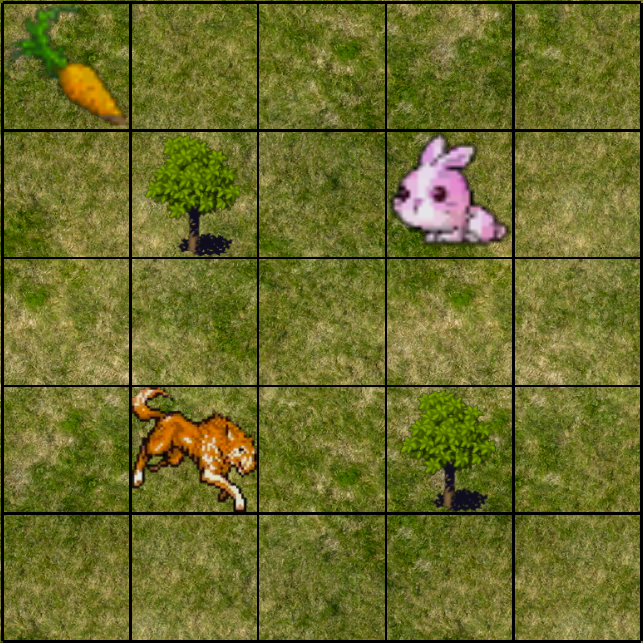
\includegraphics[height=2.4in]{bunny.png}
\end{center}


\caption{In the grid world above, the bunny must pursue two goals simultaneously: find food and avoid the wolf.  The bunny may move up, down, left, or right.  When it finds food it consumes the food and new food appears elsewhere in the grid world, when it meets the wolf it is eaten and ``respawns'' elsewhere.}
\label{fig:bunny-picture}
\end{figure}

In this task each programmer wrote an agents that control a bunny character in a simple world, depicted in Figure~\ref{fig:bunny-picture}.  The bunny world works as follows:

\begin{itemize}

\item The bunny world is a discrete grid of cells.  The bunny, wolf, and food each occupy one cell.

\item During each time step the bunny may move north, south, east, or west -- this is the bunny agent's action set.

\item Every two time steps the wolf moves towards the bunny.

\item If the bunny moves to the cell currently occupied by the food, the agent should be written to recognize this fact and give the agent an appropriate reward signal. In any case the simulation assumes food is ``eaten'' and new food appears elsewhere.

\item If the wolf moves to the cell currently occupied by the bunny it eats the bunny and the bunny ``respawns'' in a new location.

\end{itemize}

Programmers were asked to write bunny agents that meet the wolf as little as possible and eat as much food as possible.

\subsection{Task 2: Mating Bunny}\label{sec:task2}

In this task each programmer wrote a bunny agent for a world that is identical to the world in Task 1 except that the bunny must also find mates.  This world includes one static  potential mate that behaves similarly to the food.  When the bunny finds the potential mate, the simulation assumes that the bunny has ``mated,'' the mate disappears, and another potential mate appears elsewhere.  The simulation runs as in Task 1, and the scorer additionally keeps track of how many mates the bunny finds.  As in Task 1, programmers were asked to write bunny agents that meet the wolf as little as possible, eat as much food as possible, and find as many mates as possible.

%% \subsection{Task 3: Adding Wind, Spoiling Food, and Picky Mates}\label{sec:task3}

%% In this task each programmer will write a bunny agent for a world with the same elements as in Task 2 and with the same goals for the bunny, but the world is more complex.  In particular:

%% \begin{itemize}

%% \item There is constant wind from an unchanging direction that affects the wolf's ability to find the bunny.  The wolf will only move toward the bunny if the wolf is downwind of the bunny.

%% \item If food is not eaten within 15 time steps after it appears, it spoils.  Spoilage is represented by the food disappearing and new food appearing elsewhere.

%% \item To simulate selection of fit bunnies, potential mates will only accept the bunny if the bunny has eaten within 10 time steps (a hungry bunny is an unsuccessful bunny and therefore not fit for mating).  Rejection will be represented by the potential mate remaining in place and the bunny not receiving a signal that mating has occurred.

%% \end{itemize}

\subsection{Provided Code}

Study participants were given starter code so they could focus on writing the behavior of their agents. We provided the world for each task and the files in which to write their code. Participants were also given general documentation for AFABL but assumed to already be proficient in Scala.

Figure \ref{fig:scala-task1-provided} shows the code given to participants for the Scala bunny on Task 1. Figure \ref{fig:afabl-task1-provided} shows the code given to participants for the AFABL bunny on Task 1. The {\tt BunnyWorld}, {\tt BunnyState}, and {\tt BunnyAction} classes were also provided. It was up to participants to write state abstraction classes if they chose to do so.


\begin{figure}[!h]
\begin{center}

\begin{lstlisting}[language=Scala]
class ScalaBunny1 extends Agent[BunnyState, BunnyAction.Value]
    with Task1Scorer {

  // Your code goes in the body of this method. This method defines
  // your agent's behavior, that is, what action it takes in a given
  // state. The last expression in this method must be a
  // BunnyAction.  You may create as many helper functions as you
  // like, but please do not alter any of the provided code.
  def getAction(state: BunnyState, shouldExplore: Boolean = false) = {

    // This is a stub to make the code compile. Please
    // replace this with your code.
    BunnyAction.Up
  }
}
\end{lstlisting}

\caption{Starter Scala code provided to participants for Task 1.}
\end{center}
\label{fig:scala-task1-provided}
\end{figure}


\begin{figure}[!h]
\begin{center}

\begin{lstlisting}[language=Scala]
object AfablTask1 {

  // Use this val in your agent definitions.
  val bunnyWorld = new BunnyWorld

  // Please place all of your AFABL code for Task 1 in this singleton
  // object.


  // Your solution must assign your AFABL bunny agent for Task 1 to
  // the val afablBuny1.
  val afablBunny1 = ???
}
\end{lstlisting}

\caption{Starter AFABL code provided to participants for Task 1.}
\end{center}
\label{fig:afabl-task1-provided}
\end{figure}


The provided code for Task 2 was identical to the provided code for Task 1, except for the names of the files. For Task 2 participants were encouraged to copy code from Task 1 if they found it helpful, or to use any objects defined for Task 1 that would be helpful, such as behavior modules. As we discuss below, reusing code was straightforward for the AFABL agents but not for the Scala agents. As in Task 1, it was up to participants to write state abstraction classes if they chose to do so, but they could reuse any state abstraction classes written for Task 1.

Each task had a main method which ran the agents in the world to evaluate their performance.

\section{Quantitative Results}

We analyzed the submissions of study participants to compare Scala agents to AFABL agents in terms of code size, time spent writing Scala versus AFABL agents, the complexity of Scala versus AFABL agent code, and the performance of the agents on the assigned tasks.

\subsection{Code Size}

The size of a code base is often correlated with the level of effort required to write or understand the code. We computed the number of lines of code for each agent, not including comments.

\subsection{Time}

Study participants used the IntelliJ IDEA IDE with a plug-in that we wrote especially for this study. The plug-in recorded timestamps each time the editor tab with Task 1 or Task 2 files gained or lost the focus. We processed these logs to add up the time deltas between gaining and losing focus as an indication of the time programmers spent writing the code for each bunny agent.

\subsection{Cyclomatic Complexity}

We computed a complexity measure for all the submitted bunny agents. For Scala code we employed the simplified McCabe cyclomatic complexity measure \cite{mccabe1976complexity}:

\begin{equation}
v = \pi + 1
\end{equation}

where $v$ is the complexity score and $\pi$ is the number of predicates in decision structures.

\subsection{Performance}

Each programmer's Scala bunny and AFABL bunny were run for 1000 time steps and their average scores recorded. The score is based on how much food the bunny eats and how many times the bunny is eaten by the wolf for Task 1, and additionally how many times the bunny mates for Task 2. The score is normalized by the number of steps to indicate a sort of ``happiness index,'' a ratio of rewards to lifespan. This score happens to correspond to the measure used to validate Arbi-Q in Chapter \ref{ch:arbiq} to facilitate comparison between programmer authored agents and the performance of the algorithms we implemented for our reformulated MRL. It is important to note, however, that our aim here is not to achieve optimal performance but to create a programming system that makes it easy to write agents that achieve good performance.

\subsection{Typical Task 1 Submissions}

\begin{figure}[!h]
\begin{center}

\begin{lstlisting}[language=Scala]
class ScalaBunny1 extends Agent[BunnyState, BunnyAction.Value]
    with Task1Scorer {

  def getAction(state: BunnyState, shouldExplore: Boolean = false) = {
    if (wolfNearFood(state))
      moveAwayFromWolf(state)
    else
      moveTowardFood(state)
   }

  def wolfNearFood(state: BunnyState) = {
    val wolfToFood = sqrt(pow(state.food.x - state.wolf.x, 2) +
                          pow(state.food.y - state.wolf.y, 2))
    val bunnyToFood = sqrt(pow(state.food.x - state.bunny.x, 2) +
                           pow(state.food.y - state.bunny.y, 2))
    wolfToFood < bunnyToFood
  }

  def moveTowardFood(state: BunnyState) = {
    if (state.food.x > state.bunny.x)
      BunnyAction.Right
    else if (state.food.x < state.bunny.x)
      BunnyAction.Left
    else if (state.food.y < state.bunny.y)
      BunnyAction.Up
    else
      BunnyAction.Down
  }

  def moveAwayFromWolf(state: BunnyState) = {
    if (state.wolf.x < state.bunny.x)
      BunnyAction.Right
    else if (state.wolf.x > state.bunny.x)
      BunnyAction.Left
    else if (state.wolf.y > state.bunny.y)
      BunnyAction.Up
    else
      BunnyAction.Down
  }
}
\end{lstlisting}

\caption{Typical Scala submission for Task 1.}
\end{center}
\label{fig:scala-task1-submission}
\end{figure}

Figure \ref{fig:scala-task1-submission} shows a typical Scala submission for Task 1. The action selection strategy is about as simple as possible. For example, there is no determination of where the wolf is in relation to the bunny and food other than distance. If the wolf is closer to the food than the bunny, move away from the wolf, otherwise move toward to the food. The agent does not distinguish between cases where the wolf is between the wolf and the food, or if the wolf is closer but sufficiently far away. One could imagine writing code to calculate the projection of the wolf's position onto the line between the bunny and the food to determine a safe closure rate for the wolf. However, this simple strategy is all that is needed to achieve nearly optimal results. This Scala-only bunny agent achieves an average performance score of 0.54, the same as the AFABL bunny.

\begin{figure}[!h]
\begin{center}

\begin{lstlisting}[language=Scala]
  case class FindFoodState(bunny: Location, food: Location)
  val findFood = AfablModule(
    world = bunnyWorld,
    stateAbstraction = (worldState: BunnyState) => {
      FindFoodState(worldState.bunny, worldState.food)
    },
    moduleReward = (moduleState: FindFoodState) => {
      if (moduleState.bunny == moduleState.food) 1.0
      else -0.1
    }
  )

  case class AvoidWolfState(bunny: Location, wolf: Location)
  val avoidWolf = AfablModule(
    world = bunnyWorld,
    stateAbstraction = (worldState: BunnyState) => {
      AvoidWolfState(worldState.bunny, worldState.wolf)
    },
    moduleReward = (moduleState: AvoidWolfState) => {
      if (moduleState.bunny == moduleState.wolf) -0.1
      else 0.1
    }
  )

  val afablBunny1 = AfablAgent(

    world = bunnyWorld,

    modules = Seq(findFood, avoidWolf),

    agentLevelReward = (state: BunnyState) => {
      if (state.bunny == state.wolf) 0.0
      else if (state.bunny == state.food) 1.0
      else 0.5
    }
  )
\end{lstlisting}

\caption{Typical AFABL submission for Task 1.}
\end{center}
\label{fig:afabl-task1-submission}
\end{figure}

Figure \ref{fig:afabl-task1-submission} shows a typical AFABL submission for Task 1. As in our earlier examples, the AFABL bunny is composed of behavior modules for finding food and avoiding the wolf. The AFABL documentation contained tips for reward authoring in modules and at the agent level.


The AFABL solution to Task 1 contains 31 lines of code and has a cyclomatic complexity of 5 (4 predicates in decision structures). The Scala solution to Task 1 uses 34 lines of code and has a cyclomatic complexity of 8 (7 predicates in decision structures). Both programs achieve the same nearly optimal level of performance with scores of ~0.54.

\subsection{Typical Task 2 Submissions}

\begin{figure}[!h]
\begin{center}

\begin{lstlisting}[language=Scala]
class ScalaBunny2 extends Agent[BunnyState, BunnyAction.Value]
    with Task2Scorer {

  def getAction(state: BunnyState, shouldExplore: Boolean = false) = {

    if ((distance(state.wolf, state.food) < distance(state.food, state.bunny))
      || distance(state.wolf, state.mate) < distance(state.mate, state.bunny))
      moveAwayFromWolf(state)
    else if (distance(state.bunny, state.food) < distance(state.bunny, state.mate))
      moveToward(state.bunny, state.food)
    else
      moveToward(state.bunny, state.mate)
  }

  def distance(a: Location, b: Location) = {
    sqrt(pow(a.x - b.x, 2) + pow(a.y - b.y, 2))
  }

  def moveToward(from: Location, to: Location) = {
    if (to.x > from.x)
      BunnyAction.Right
    else if (to.x < from.x)
      BunnyAction.Left
    else if (to.y > from.y)
      BunnyAction.Up
    else
      BunnyAction.Down
  }

  def moveAwayFromWolf(state: BunnyState) = {
    if (state.wolf.x < state.bunny.x)
      BunnyAction.Right
    else if (state.wolf.x > state.bunny.x)
      BunnyAction.Left
    else if (state.wolf.y > state.bunny.y)
      BunnyAction.Up
    else
      BunnyAction.Down
  }
}
\end{lstlisting}

\caption{Typical Scala submission for Task 2.}
\end{center}
\label{fig:scala-task2-submission}
\end{figure}

Figure \ref{fig:scala-task2-submission} shows a typical Scala solution for Task 2. While the Scala solution to Task 2 is more complex than the Scala solution to Task 1, it uses only one more line of code -- 35 -- due to refactoring of common logic. Of course, this refactoring took extra time and without the refactoring the line count and likely the cyclomatic complexity would have been higher.

\begin{figure}[!h]
\begin{center}

\begin{lstlisting}[language=Scala]
  case class FindMateState(bunny: Location, mate: Location)
  val findMate = AfablModule(
    world = bunnyWorld,
    stateAbstraction = (state: BunnyState) => {
      FindMateState(state.bunny, state.mate)
    },
    moduleReward = (state: FindMateState) => {
      if (state.bunny == state.mate) 1.0
      else -0.1
    }
  )

  // Your solution must assign your AFABL bunny agent for Task 2 to
  // the val afablBuny2.
  val afablBunny2 = AfablAgent(

    world = bunnyWorld,

    modules = Seq(AfablTask1.findFood, AfablTask1.avoidWolf, findMate),

    agentLevelReward = (state: BunnyState) => {
      if (state.bunny == state.wolf) 0.0
      else if (state.bunny == state.food) 1.0
      else if (state.bunny == state.mate) 1.0
      else 0.5
    }
  )
\end{lstlisting}

\caption{Typical AFABL submission for Task 2.}
\end{center}
\label{fig:afabl-task2-submission}
\end{figure}

Figure \ref{fig:afabl-task2-submission} shows typical AFABL code for Task 2. Notice that the {\tt findFood} and {\tt avoidWolf} modules from Task 1 have been reused directly. This works because the world, {\tt BunnyWorld}, is the same. In Task 1 the bunny was ignoring the mate. In Task 2 we adapt the bunny to find the mate, and all we need to do is add a {\tt findMate} module and add a line to the {\tt agentLevelReward} function so that the agent will also value finding mates.

The AFABL solution to Task 2 contains 21 lines of code due to reuse of modules from Task 1, and has the same cyclomatic complexity of 5 (4 predicates in decision structures) even though the agent is solving a more complex problem. Even with the refactoring of common logic in Task 2 the Scala solution has a higher cyclomatic complexity of 10 (9 predicates in decision structures), which McCabe says is the maximum allowable cyclomatic complexity for a testable, maintainable software module \cite{mccabe1976complexity}. Finally, the performance of the Scala solution to Task 2 decreases to 0.48, while the AFABL solution continues to achieve the same nearly optimal 0.54. With additional work perhaps the Scala agent's performance on Task 2 could have been improved, but the point here is that AFABL agents are easier to write, easier to adapt to new domains, have less complex code, and perform well without requiring a great deal of effort beyond choosing reward signals.

\subsection{Summary}

TBD ...

Quantitative results for Task 1 are summarized in Table \ref{tbl:task1-results}. Quantitative results for Task 2 are summarized in Table \ref{tbl:task2-results}.

\begin{center}
\begin{table}[h]
\begin{tabular}{|l|r|r|r|}\hline
                      & Scala Mean & AFABL Mean & p-value \\\hline
Lines of Code         & 0.0        & 0.0        & 0.0 \\
Time                  & 0.0        & 0.0        & 0.0 \\
Cyclomatic complexity & 0.0        & 0.0        & 0.0 \\
Performance           & 0.0        & 0.0        & 0.0 \\\hline
\end{tabular}
\caption{Quantitative results of Scala agent code versus AFABL agent code on Task 1. A p-value of less than .05 mean that the difference in means is statistically significant at the 95\% significance level, i.e. we reject $H_0: \mu_1 = \mu_2$ and conclude that the means are different.}
\label{tbl:task1-results}
\end{table}
\end{center}

\begin{center}
\begin{table}[h]
\begin{tabular}{|l|r|r|r|}\hline
                      & Scala Mean & AFABL Mean & p-value \\\hline
Lines of Code         & 0.0        & 0.0        & 0.0 \\
Time                  & 0.0        & 0.0        & 0.0 \\
Cyclomatic complexity & 0.0        & 0.0        & 0.0 \\
Performance           & 0.0        & 0.0        & 0.0 \\\hline
\end{tabular}
\caption{Quantitative results of Scala agent code versus AFABL agent code on Task 2. A p-value of less than .05 mean that the difference in means is statistically significant at the 95\% significance level, i.e., we reject $H_0: \mu_1 = \mu_2$ and conclude that the means are different.}
\label{tbl:task2-results}
\end{table}
\end{center}

\section{Qualitative Results}

TBD ...

Programmers responded to a questionnaire to give their impressions of agent programming in AFABL versus agent programming in Scala.

\begin{enumerate}
\item I have a positive impression of agent programming in Scala.

Rationale: programmers’ impression of Scala will provide a baseline for evaluating
programmers’ impression of AFABL.

\item I found it easier to write the agents using AFABL’s programming constructs compared to bare Scala.

Rationale: the point of AFABL is to facilitate agent programming, so programmers should have a more positive impression of AFABL for agent programming.

\item I believe that AFABL facilitated more reusable and maintainable code for agents compared to bare Scala.

Rationale: answers to this question should correlate with answers to Question 1.

\item If given the choice, I would choose AFABL over Scala for agent programming projects.

Rationale: answers to this question should correlate with answers to Question 2.

\item I found it easier to use AFABL compared to Scala for Task 1.

  Rationale: in addition to objective analyses of task submissions, we want to know whether programmers subjectively prefer AFABL.

\item What was it about AFABL that made the Task 1 easier or harder?

Rationale: we want to get open-ended feedback for things we did not anticipate.

\item I found it easier to use AFABL compared to Scala for Task 2.

Rationale: in addition to objective analyses of task submissions, we want to know whether programmers subjectively prefer AFABL.

\item What was it about AFABL that made the Task 2 easier or harder?

\end{enumerate}

\section{Conclusion}

As you can see from the similarity of the submission in Figure \ref{fig:afabl-task1-submission} to our explanatory example, most AFABL bunny agents look the same. There is one obvious way to implement a bunny agent that must pursue multiple goals. This uniformity is desirable. As Tim Peters says in the Zen of Python \cite{peters2004zen}, ``There should be one-- and preferably only one --obvious way to do it.'' The similarity in most AFABL solutions to a particular modular agent programming problem is an indication that AFABL provides the right abstractions for adaptive agent programming.


\chapter{An Example Application: Deriving Behavior from Personality}\label{ch:applications}

In this chapter we present an application of language-integrated reinforcement learning to the problem of personality simulation. Creating artificial intelligent agents that are high-fidelity simulations of natural agents will require that behavioral scientists be able to write code themselves, not merely act as consultants with the ensuing knowledge acquisition bottleneck. However, translating personality models into the concrete behavior of an agent using currently available programming constructs would require a level of code complexity that would make the system inaccessible to behavioral scientists.  What we need is a way to derive the concrete actions of an agent directly from psychological personality models.  This chapter describes a reinforcement learning approach to solving this problem in which we represent trait-theoretic personality models as reinforcement learning agents.  We validate our approach by creating a virtual reconstruction of a psychology experiment using human subjects and showing that our virtual agents exhibit similar behavior patterns. Note that this work was conducted and published before we finished the Arbi-Q command arbitration algorithm of Chapter \ref{ch:arbiq}, so the AFABL agents used the Greatest-Mass q-decomposition algorithm. We have also updated the code from our original work to use AFABL syntax.


\section{Introduction}

There is tremendous interest in creating synthetic agents that behave as closely as possible to natural (human) agents.  Rich, interactive intelligent agents will advance the state of the art in training simulations, interactive games and narratives, and social science simulations.  However, the programming systems for creating such rich synthetic agents are too complex, or rather too steeped in computational concepts, to be used directly by the behavioral scientists who are most knowledgeable in modeling natural agents. Engaging behavioral scientists more directly in the authoring of synthetic agents would go a long way towards improving the fidelity of synthetic agents.

What we need is a programming language that a behavioral scientist can use to write agent programs using concepts familiar to behavioral scientists.  This task is complicated by the fact that the most popular and best understood personality models from behavioral science do not lend themselves to direct translation into computer programs.  Requiring a behavioral scientist to specify behaviors in the detail required in even the most cutting edge purpose-built programming language would plunge the would-be behavioral scientist agent programmer right into a morass of complex computational concepts that lie outside the expertise of most dedicated behavioral experts. To solve this problem we need a way to get from personality models to behaviors, to derive specific agent actions in an environment from a personality model without having to program the derivation in great detail.

In this chapter, we describe a way to model motivational factors from trait-oriented personality theory with reinforcement learning modules.  We describe a virtual agent simulation that reconstructs a human subject experiment from psychology, namely some of Atkinson's original work in achievement motivation and test anxiety, and show that our simulation exhibits the same general behavior patterns as the human subjects in Atkinson's experiments.  First, we briefly discuss relevant personality research and provide some background.

\subsection{Personality}

Personality is a branch of psychology that studies and characterizes the underlying commonalities and differences in human behavior. Within psychology, there are two broad categories of personality theories: processing theories, and dispositional, or trait theories. Social-cognitive and information-processing theories identify processes of encodings, expectancies, and goals in an attempt to characterize the mechanisms by which people process their perceptions, store conceptualizations, and how those processes drive their interactions with others \cite{dweck1988a-social-cognitive,cervone2009personality,cervone1999the-coherence}. A strength of processing theories, especially from a computational perspective, is that they provide a detailed account of the cognitive processes that give rise to personality and drive behavior.  This strength is also a drawback -- processing theories tend to be detailed and often low-level (though not as low-level as cognitive architectures, which we will discuss below), and this makes them less intuitive and less suited to describing personality in broad, easily understood terms.

Trait theories \cite{cervone2009personality}, the most well-known example of which is the Five-Factor model \cite{mccrae2008handbook}, attempt to identify stable traits (sometimes called ``trait adjectives'') that can be measured on numerical scales and remain invariant across situations in determining behavior.  A strength of the trait approach is that they are well-suited to describing individuals in broad, intuitive terms.  Two drawbacks of the approach are that there is not yet widespread agreement on a set of truly universal traits (or how many there are), and it is not clear how trait models drive behavior.  A promising line of research by Elliot and Thrash \cite{elliot2002approach-avoidance} is working towards solving these problems by integrating motivation into personality in a general way.  The work of Elliot and Thrash particularly supports the approach we present here, as they show that approach and avoidance motivation underpins all currently popular trait theories.

While debate continues about the merits and drawbacks of the different approaches to personality, the psychology community is also attempting to unify personality and motivation theory \cite{mischel2008handbook}. While the work we present here is focused on bridging the gap between the descriptive power of trait-oriented models and the behavior that arise from them, we consider this work to be complementary to work in encoding information processing theories.  In the future, rich computational agents may be built by combining approaches.

\subsection{Modeling Personality with Reinforcement Learning}

The essential idea behind modeling personality traits with reinforcement learning is that each motivational factor can be represented by a reinforcement learning module.  In psychology, the inherent desirability or attractiveness of a behavior or situation is referred to as {\em valence}.  For a person high in success approach motivation, behaviors or situations that provide an ``opportunity to excel'' will have high valence, while other behaviors will have lower valence.  The notion of valence translates fairly directly into the concept of reward in reinforcement learning.  Just as people with certain motivational factors will be attracted to high-valence behaviors, a reinforcement learner is attracted to high-reward behaviors.  This is the basis for modeling motivational factors with reinforcement learning modules.  By encoding the valence of certain behaviors as a reward structure, reinforcement learners can learn the behavioral patterns that are associated with particular motivational factors.  This is a powerful idea, because it allows an agent author to write agent code using motivational factors while minimizing the need to encode the complex mechanisms by which such factors lead to concrete behavior.

A critical aspect of trait theory is that traits can have interactive effects.  It is clear that a person who is high in achievement motivation will ``go for it'' when given the opportunity and that a person who is high in avoidance motivation will be more reserved.  But what happens when a person is high in both motivations?  Such interactive effects cannot be ignored in a credible treatment of personality, but it is hard to predict the behavioral patterns that will arise from given combinations of motivational factors.  One can imagine the code complexity that might result from trying to model such interactive effects with production rules or other traditional programming constructs.  As we demonstrate later, our reinforcement learning approach handles such interactive effects automatically.

It is important to note that we are not creating a new theory of personality.  We are creating a computational means of translating existing theories of personality from {\em psychology} (not computer science) into actions executed by synthetic agents.  We are also not committing to a particular theory from psychology, but rather supporting the general category of trait theories of personality which, until now, have not been directly realizable in computer agents.

In the remainder of this chapter we discuss some related work in agent modeling, present our virtual reconstruction of a human subject experiment using our reinforcement learning approach, and discuss the promising results and their implications for future work.


\section{Related Work}\label{sec:related-work}

There is a great deal of work in modeling all sorts of phenomena in synthetic agents.  Cognitive architectures provide computational models of many low-level cognitive processes, such as memory, perception, and conceptualization \cite{jones2005an-introduction,langley2008cognitive}.  Cognitive architectures support scientific research in cognitive psychology by providing runnable models of cognitive processes, support research in human-computer interaction with detailed user models \cite{john1998cognitive}, and can serve as the ``brains'' of agents in a variety of contexts.  The most notable and actively developed cognitive architectures are Soar \cite{laird2008extending} and ACT-R \cite{anderson2004an-integrated}.  Recently, some effort has gone into integrating reinforcement learning into Soar \cite{nason2008soar-rl}.  While RL is used to improve the reasoning system in Soar, we are using RL to support new paradigms of computer programming for agent systems.  In general, our work differs from and complements work in cognitive architectures in that we are drawing on psychological theory that is expressed at a much higher level of abstraction.  Cognitive psychology and AI have often built on each other.  Indeed, cognitive psychology is the basis of cognitive architectures in AI.  Our work is an attempt to bring in mainstream personality psychology as a basis for building intelligent agents, which we hope will complement the detailed models of cognitive architectures in creating rich synthetic agents.

There is a large and rich body of work in believable agents.  Mateas and Stern built on the work of the Oz project \cite{loyall1991hap} in creating a programming language and reactive--planning architecture for rich believable agents. They implemented their theory in the computer game Facade, a one-act interactive drama in which the player interacts with computer simulated characters that provide rich social interactivity \cite{mateas2004life-like}.  Gratch, Marsella and colleagues have a large body of work in creating rich simulations of humans for training simulations that incorporate models of appraisal theory and emotion \cite{gratch2005lessons,swartout2006toward}.  A distinctive feature of the work of both Mateas, et. al., and Gratch, et. al., is that they are dealing with the entire range of AI problems in creating believable agents that sense, act, understand and communicate in natural language, think, and exhibit human-like personalities.  Our work differs from other work in personality modeling in that we are not attempting to simulate personality, but using definitions of personality to drive the behavior of synthetic agents.  We want to derive behavior that is consistent with a given personality model, but not necessarily to ensure that the agent gives the appearance of having that personality.


\section{Experiments}

To test our claim that personality can be modeled by reinforcement learning modules, we created a population of simple two-module multiple-goal reinforcement learning agents and ran them in a world that replicated experiments carried out with humans by psychologist John Atkinson.  First we describe Atkinson's original research, and then discuss our virtual reconstruction of his experiments.

\subsection{Atkinson's Ring Toss Experiment}\label{sec:ring-toss}

John Atkinson was among the first researchers to study the existence and role of approach and avoidance motivation in human behavior. Prior to Atkinson's work, it was believed that test anxiety was equivalent to low achievement motivation.  However, Atkinson showed that test anxiety is actually a separate avoidance motivation, a ``fear of failure'' dimension that works against and interacts with achievement motivation \cite{atkinson1960achievement}.  To test his hypothesis, he administered standard tests of achievement motivation and test anxiety to a group of undergraduate psychology students and devised a series of experiments which examined the effort put forth in achieving success in tasks such as taking a final exam.  It is important to note that he did not measure the outcomes of the task, but rather the effort put forth in doing well in them.  Thus, his experiments examined the relationship between motivation and {\em behavior}, not necessarily competence.  One of his experiments, a ring toss game, produced results that clearly show the interplay of approach and avoidance motivation and is particularly well-suited to computer simulation.

In Atkinson's ring toss experiment, subjects played a ring toss game in which players attempted to toss a ring from a specified distance onto a peg.  Subjects made 10 tosses from any distance they wished, from 1 through 15 feet, and the distance at which each subject made each toss was recorded.  For analysis, subjects were divided into four groups according to their measures of achievement motivation and test anxiety so that the relationship between these motivations and their behavior could be analyzed.  For each of the two measures -- achievement motivation and test anxiety -- subjects were classified as either high or low, with the dividing line between high and low set at the median scores in each measure.  (For example, a H-L subject is high in achievement motivation and low in test anxiety).  Subjects were divided into four groups -- H-L, H-H, L-L, and L-H -- and the percentage of shots taken at each distance by each group was recorded. We discuss his results and our simulation below.

\subsection{Computational Models of Atkinson's Subjects}

We reconstructed Atkinson's ring toss experiment in a computer simulation.  We created 49 virtual agents that corresponded to each of the 49 human subjects in Atkinson's experiments, with the same distribution of high and low measures of achievement motivation and test anxiety.  Simplified code for a representative student subject is presented in Figure \ref{fig:student}.  Since we did not have access to Atkinson's source data, we modeled high motivation measures as having a mean of 1.5 and low motivation with a mean of 0.5, both with standard Normal distributions (mean = 0, variance = 1) scaled by $\frac{1}{2}$, so virtual test subjects did not all have the same measures.

\begin{figure}[h]

\begin{lstlisting}
val motivatedStudent = GmAgent(
  world = RingTossWorld,

  // Sequence of pairs where the second element of each pair
  // is the weight of the pair, corresponding to the personality
  // trait measure
  modules = Seq((achievementMotivation, 1.5 + X ~ N(0, 1) / 2),
                (testAnxiety, .5 + X ~ N(0, 1) / 2))
}
\end{lstlisting}

\caption{An agent representing a success-oriented student in Atkinson's ring toss experiment, containing two RL modules representing high achievement motivation and low test anxiety.  The code snippets presented here are simplified versions of the Scala code we used to run our experiments.}
\label{fig:student}
\end{figure}

As discussed earlier, each of the motivational dimensions of the virtual subjects was implemented with reinforcement learning modules that learned to satisfy the preference for perceived valence of behaviors (modeled as reward).  For example, in the achievement motivation module (see Figure \ref{fig:achievement}), the greater the distance from the peg, the greater the reward because it represents greater achievement.  Similarly, in the test anxiety module (see Figure \ref{fig:testanxiety}), greater reward is given to closer distances, because they minimize, or ``avoid'' the chance of failure from a long-distance toss.

\begin{figure}[h]
\begin{lstlisting}
val achievementMotivation = AfablModule(

  world = RingTossWorld,

  moduleReward = (state: RingTossState) => state match {
    case OneFootLine => 1,
    case TwoFootLine => 2,
    ...
    case FifteenFootLine => 15
  }

)
\end{lstlisting}
\caption{A reinforcement learning module representing achievement motivation.}
\label{fig:achievement}
\end{figure}

\begin{figure}[h]

\begin{lstlisting}
val testAnxiety = AfablModule(

  world = RingTossWorld,

  moduleReward = (state: RingTossState) => state match {
    case OneFootLine => 15,
    case TwoFootLine => 14,
    ...
    case FifteenFootLine => 1
  }

)
\end{lstlisting}

\caption{A reinforcement learning module representing Test Anxiety (`avoidance motive, a.k.a. ``fear of failure'').  Note that the rewards are inverted from the achievement motivation module, that is, the valence of avoiding achievement is higher.}
\label{fig:testanxiety}
\end{figure}

Internally, each personality module is implemented with the standard Q-learning algorithm \cite{sutton1998reinforcement}.  The ring toss world consists of 16 states -- a start state and one state for each of the 15 distances, and 15 actions available in each state that represent playing (making a toss) from a particular distance.  Each reinforcement learning module used a step-size parameter of $\alpha = 0.1$, a discount factor of $\gamma = 0.9$ (though discounting wasn't important given that the 15 states representing playing lines were terminal states, since each play was a training episode), and employed an $\epsilon$-greedy action selection strategy with $\epsilon = 0.2$.  (Readers familiar with reinforcement learning will also notice that this game is equivalent to a 15-armed bandit problem.)  We emphasize that the details of the reinforcement learning algorithms are not essential to modeling motivational factors, and those details are hidden inside the implementation of the modules.  Indeed a major goal of our work is to simplify the task of writing synthetic agents by taking care of such details automatically.

Recall that reinforcement learning algorithms learn an action value for each action available in a given state.  An action value for a state represents the expected total reward that can be achieved from a state by executing that action and transitioning to a successor state. For each of the modules -- Achievement and TestAnxiety -- the action values represent the learned utility of the actions in serving the motivational tendencies the modules represent.  The Student agents take into account the preferences of the modules -- represented by action values -- by summing their action values weighted by their module weights to get a composite action value for each action in a given state.  If we denote each module's action value by $Q(s, a)$ and the weights by $W$, then the composite, or overall, action value is:

\begin{align}
Q_{student}(s,a) =  & W_{Achievement} Q_{Achievement}(s,a) +\\
                   & W_{TestAnxiety} Q_{TestAnxiety}(s,a)
\end{align}

For the virtual experiments, each module -- Achievement and TestAnxiety -- was run to convergence and then the student agents simulated 10 plays of the ring toss game, just as in Atkinson's experiment.  We discuss the results of the experiment below.

\section{Model Validation}

A model is a set of explicit assumptions about how some system of interest works \cite{law2007simulation}.  In psychology the system of interest is (usually) a human or group of humans.  Our virtual reconstruction of Atkinson's experiments constitutes a computational representation of Atkinson's two-factor model of personality.  Thus, our agents are simulation models of Atkinson's subjects (the students in his ring toss experiment).  While the work presented here is only a proof of concept, we do hope to achieve a high level of validity as we refine our approach, so it will be useful to validate our models using techniques from simulation science \cite{law2007simulation}.

As we described earlier, Atkinson divided his subjects into four groups according to their measures (high or low) on achievement motivation and test anxiety.  For each of these four groups -- H-L, H-H, L-L, L-H -- he recorded the percentage of shots that each group took from each of the 15 distances.  We ran 10 replications of our simulation and recorded the mean percentages for each group and distance.  For each percentage mean we calculated a 95\% confidence interval.  We consider a model to be valid if the confidence intervals calculated on the simulation percentage means contain the percentages obtained by Atkinson in his experiments with human subjects.

\begin{table*}[ht]
\caption{Validation Results.  For each subject group the percentage of shots taken by Atkinson's human subjects and by our simulation from each of three ranges is presented along with a 95\% confidence interval for the mean percentage of shots in 10 simulated replications of Atkinson's experiment.}

\begin{center}

\begin{tabular}{|l||c|c|c|c|} \hline
Achievement: & High & High & Low & Low \\
Test Anxiety: & Low & High & Low & High \\  \hline
 & Atkinson & Atkinson & Atkinson & Atkinson \\
 & Simulation & Simulation & Simulation & Simulation \\
Range & Conf. Int. & Conf. Int. & Conf. Int. & Conf. Int. \\ \hline\hline
  1-7 & \bf{11}           & 26              & 18           & 32 \\
      & \bf{7.7}          & 14.0            &  5.6         &  8.5 \\
      & \bf{(4.0, 11.4)}  & (5.6, 22.4)     & ( 1.4,  9.7) & ( 4.4, 12.5)\\ \hline
8-12  & \bf{82}           & 60               & 58           & 48 \\
      & \bf{75.4}         & 69.0             & 74.4         & 80.0 \\
      & \bf{(65.1, 85.7)} & (61.1, 76.9)     & (62.0, 86.9) & (74.1, 85.9)\\ \hline
13-15 & 7                 & \bf{14}           & \bf{24}           & 20 \\
      & 16.9              & \bf{17.0}         & \bf{20.0}         & 11.5 \\
      & ( 8.8, 25.0)      & \bf{(9.4, 24.6)}  & \bf{(8.3, 31.7)} & ( 6.9, 16.2)\\ \hline
\end{tabular}
\label{tab:results}

\end{center}
\end{table*}

The validation results are presented in Table \ref{tab:results}. Atkinson analyzed his experimental data by aggregating the shots taken by subjects into three ``buckets'' representing low, medium, and high difficulty.  In Atkinson's analyses the dividing lines between the three buckets were set in four different ways with each yielding similar results.  For brevity we present the division obtained by using both geographical distance and distribution of shots about the median shot of 9.8 ft, in other words, the dividing line one would choose by inspecting the histogram for distinct regions.  This strategy resulted in the three buckets listed in the left column of Table \ref{tab:results}.  Each cell of the four subject groups -- H-L, H-H, L-L, L-H - contains the percentage of shots taken by Atkinson's subjects, the mean percentage obtained by running 10 replications of our simulation of Atkinson's experiment, and a 95\% confidence interval for the mean percentage.  While our model did not achieve formal validation, the general patterns of behavior are quite similar to Atkinson's human subject experiment, as shown in Figure \ref{fig:ring-toss-plots}, and we consider these results to be a good proof of concept.  We discuss some reasons behind these results and strategies for improvement below.

%% 8< 8< 8< 8< 8< 8< 8< 8< 8< 8< 8< 8< 8< 8< 8< 8< 8< 8< 8< 8< 8< 8< 8<

\begin{figure}[!h]
  \begin{center}
    \scalebox{.8}{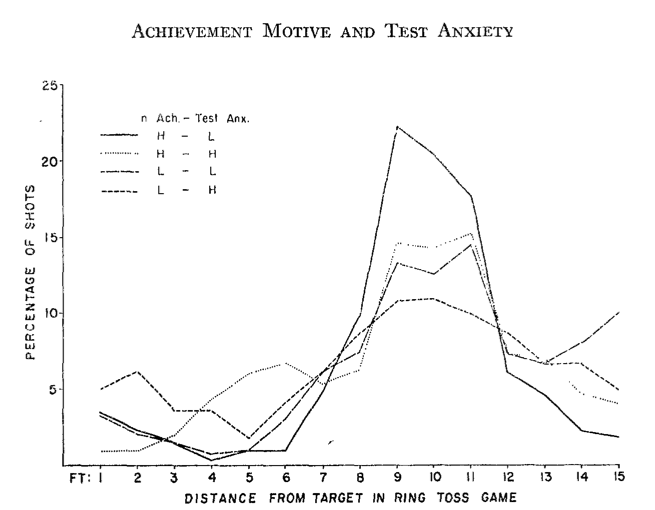
\includegraphics{atkinson}}
    \scalebox{.4}{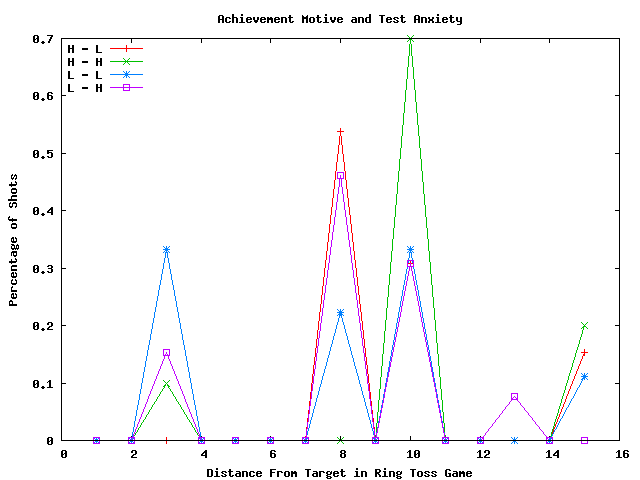
\includegraphics{iccm}}
    \caption{The top plot shows the behavior patterns of human
      subjects in Atkinson's Ring Toss experiment.  The bottom plot
      shows the behavior patterns of our synthetic agents that
      re-created Atkinson's experiment.  Note that Atkinson's plot is
      smoothed, while ours is not.}
  \end{center}
  \label{fig:ring-toss-plots}
\end{figure}

%% 8< 8< 8< 8< 8< 8< 8< 8< 8< 8< 8< 8< 8< 8< 8< 8< 8< 8< 8< 8< 8< 8< 8<

\section{Discussion}

We made several assumptions in our models that affected the validation results.  First, because we did not have access to Atkinson's original data, only summary presentations, we did not know the exact distribution of motivational factors among his subjects, or even the scales used in his measures.  We assumed normally distributed measures and tried several different scales before settling on the values used in the simulations reported here.  Second, it is not clear how the valence of behaviors should be translated into reward structures for RL agents.  We chose a simple linear reward structure in hopes that the system would be robust to naive encodings.  To make our approach widely useful we will need to address the manner in which reward structures are determined.

%% Third, we calculated aggregate action values by a simple weighted sum of module action values.  We are currently investigating optimal arbitration of multiple RL modules and hope to report results within the next six months.

We chose the Atkinson ring toss experiment on the advice of psychologists who recommended it as a well-known example of trait-oriented behavior theory, and because of its simplicity. However, our goal is to create large agent systems, so future work will need to address scalability -- to greater numbers of trait factors and more complex worlds -- and generalizability, or transferability, to other domains.

%% More generally, there are broader issues to be understood about
%% employing this method in practice.  From the psychology perspective, we
%% need to understand how motivational factor scales translate into the
%% weights on reinforcement learning modules, e.g., they must be
%% normalized somehow.  This issue is similar to the issue of reward
%% comparability in reinforcement learning (discussed below).  Also, our
%% example used two motivational factors.  How do we scale this approach
%% to multiple factors?  Many trait theories contain fewer traits that
%% subsume traits in other, more detailed trait theories.  We would
%% expect such decompositions to be helpful in our formulation as well.

%% The reinforcement learning algorithm employed in these experiments
%% were standard Q-learners.  While these algorithms worked well on this
%% limited problem, they likely will not be appropriate for every
%% problem.  Indeed the No Free Lunch Theorem \cite{ho2001simple} informs
%% us that each task must be matched to an appropriate algorithm -- there
%% is no universal solution to every problem.  How do we characterize the
%% matching of reinforcement learning algorithms to particular agent
%% designs and virtual worlds?

%% The algorithms we used also employed no optimization.  Reinforcement learning suffers from the curse of dimensionality, and many techniques are being actively pursued to cope with the size of state spaces for realistic-size domains.  Profitably employing reinforcement learning in agent programming systems will mean integrating scaling techniques such as function approximation (e.g., of action-value functions or state spaces) and decomposition techniques.

Finally, notice that the example code presented in this paper contains no logic for implementing behavior.  The agents and the modules are defined declaratively by specifying a state space, an action set, and a reward structure.  The run-time system derives the concrete behavior of the agents automatically from these specifications.  This technique, sometimes called partial programming or adaptive programming\cite{simpkins2008towards}, is a key concept that increases the usability of agent programming by allowing programmers to specify {\em what} an agent is to do without getting mired in {\em how} the agent should do it.

\section{Conclusions and Future Work}

Much work remains to make accessible personality-based agent programming systems a reality, and our work is progressing on three paths.  First, the integration of reinforcement learning into agent programming systems needs to be studied further so that we know when it is useful and how much detail can be hidden from the agent programmer. This dissertation has confirmed what we already know, namely, that authoring reward functions is not straightforward. We need to be able to specify modules in simpler terms and let the reward structure be derived automatically (we will discuss this further in Chapter \ref{ch:conclusion}. Second, the examples presented here were written together so that the reward signals of each agent were directly comparable, which allowed us to use the Greatest-Mass q-decomposition algorithm for combining the modules. Now that we have an arbitration algorithm that is robust to incomparable reward scales, we can either use a {\tt GmAgent} for personality modeling, as we have done here, or extend AFABL with weighting to enable trait-oriented personality modeling. Finally, while AFABL is currently able to handle the personality modeling presented in this chapter, AFABL is still a shallowly-embedded Scala DSL and therefore beyond the programming capabilities of most psychologists. We will need to make AFABL simpler to use. Nevertheless, reinforcement learning provides a promising approach to modeling personality traits and motivational factors in synthetic agents.  In particular, it provides us with a means to create agent programming systems that are at least comprehensible by behavioral scientists and harness their knowledge directly while minimizing the need for complex programming.


\chapter{Conclusion}\label{ch:conclusion}

\section{Review of Major Contributions}

This dissertation has reported on two primary contributions: a command arbitration algorithm for robust modular reinforcement learning, and a domain-specific language that integrates modular reinforcement learning, AFABL. The benefits of language-integrated reinforcement learning have been demonstrated in a study of programmers' solutions to agent programming tasks using AFABL compared to using a traditional programming language. AFABL agents are easier to write, are expressed in less complex code, and have more readily reused components than agents written in traditional programming languages. In the remainder of this chapter we discuss some implications of AFABL (as a representative first step in language-integrated modular reinforcement learning), limitations of the current work, and directions for future work.

\section{Limitations of Current Work}

% The work presented here is promising, but focused in scope.

\subsection{Reward Authoring}

As many other researchers have noted, reward authoring is not straightforward for programmers not trained in reinforcement learning. Study participants spent much of their AFABL writing time trying out different reward structures in an effort to improve their agents' performance. Although we provided documentation with hints on how to author reward structures, writing good reward functions is too opaque for most programmers. In the next section we discuss a possible improvement to AFABL which would relieve programmers from writing the reward functions of modules.

\subsection{Training}

Using any reinforcement learning-based programming system requires the availability of a simulation environment to train the learning modules before being used ``in production.'' Using an untrained reinforcement learning agent and accepting that it will perform poorly until it learns is not practical because reinforcement learning algorithms typically require hundreds or thousands of iterations to reach an acceptable level of performance. Separate modules with local state abstractions and reward functions help speed up training, but finding good factorizations into modules is a potentially steep burden to place on the programmer for larger agents.

\subsection{Host Language Limitations}

Writing AFABL agents is writing Scala code, so AFABL programmers must have at least basic competence with Scala and the Scala tool chain. Since it was outside the scope of the present work, we did not try to determine how much of the Scala tooling can be hidden or automated for AFABL programmers. We required study participants to use a recent version of IntelliJ IDEA and provided a pre-configured Scala/AFABL project and an IntelliJ plugin to automate the time tracking and submission process. Still, several participants had trouble running the study code smoothly, as is often the case with development tools. Many study participants who did not participate in a group session simply abandoned the study. We advertised the study to the Atlanta Scala Meet-up, a group of local software engineers either using Scala professionally or interested in learning. Approximately 15 Scala Meet-up members started the study and only one finished. Due to the number of individual software issues we needed to help participants solve -- differing operating systems, IntelliJ versions, etc -- we believe many of these dropouts were due to simple software setup issues.

In addition to Scala tooling issues, AFABL programmers must deal with the Scala programming language. For example, when a programmer makes a mistake in their code the error messages come from the Scala compiler and run-time system, not AFABL. Luckily, in the study few people had such issues with AFABL code itself. With more complex agents problems are more likely to occur, and the programmer may be faced with the famous complexity of the Scala type system. The AFABL programmer who is not also a competent Scala programmer has little hope of debugging non-trivial errors.

\section{Directions for Future Work}


\subsection{Refined Module Types}

AFABL currently supports a narrow definition of an agent: a behaving entity with a set of states that must constantly be pursued or avoided. In reinforcement learning these kinds of modules are called called continuing tasks, as opposed to episodic goals. Previous versions of AFABL supported a greater set of features but we removed them to focus on AFABL's core for the purpose of this work. With a cleaner core AFABL we could re-implement some of these features and more, which we discuss below.

\paragraph{Drives}

A Drive is a behavior module that runs throughout the life of its containing agent and represents a state that an agent should constantly seek.

\paragraph{Aversions}

An Aversion module is a behavior module that runs throughout the life of its containing agent and represents a state that an agent should constantly avoid.  It is a constraint in the sense that, in certain states, a constraint module will identify actions that should *not* be executed.

\paragraph{Objectives}

A an objective is a short-term goal state that generates a drive module that is active until its goal is achieved.  The command arbitrator gives objective modules priority over drive modules, but all modules are constrained by constraint modules.

\paragraph{Tasks}

A task is a temporally-extended action, a "mini-policy" that achieves a subgoal.  Tasks are equivalent to subtasks (MaxQ), abstract machines (PHAM), or options from hierarchical reinforcement learning. Tasks could be manually authored, or algorithms from hierarchical reinforcement learning could be integrated into AFABL.

\subsection{Simplified Syntax}

The features listed above may make it possible to automatically author reward functions for modules. For example, the Bunny agent for Task 2 from Chapter \ref{ch:afabl} could be written with Drives and Aversions as shown in Figure \ref{fig:simplified-afabl}


\begin{figure}[!h]
\begin{center}

\begin{lstlisting}[language=Scala]
  val afablBunny2 = AfablAgent(

    world = bunnyWorld,

    drives = Drives(state: BunnyState) {
      (state.bunny == state.food),
      (state.bunny == state.mate)
    },

    aversions = Aversions(state: BunnyState) {
      (state.bunny == state.wolf)
    }

    agentLevelReward = (state: BunnyState) => {
      if (state.bunny == state.wolf) 0.0
      else if (state.bunny == state.food) 1.0
      else if (state.bunny == state.mate) 1.0
      else 0.5
    }
  )
\end{lstlisting}

\caption{Simplified AFABL syntax with drives and aversions.}
\end{center}
\label{fig:simplified-afabl}
\end{figure}


Instead of writing code to specify modules, the programmer specifies states that are to be constantly sought or avoided -- expressed as state predicates -- and the modules are derived from them automatically. Note also that this proposed syntax does not include state abstraction functions in modules because they could be derived automatically from the states that are to be sought or avoided.

\subsubsection{Drama Manager Support}

The features discussed above would go along way toward supporting drama managers for intelligent interactive narratives. In addition, a drama manager would need to be able to activate and deactivate modules and inject new objectives to support particular story goals.

\subsection{General Agent Architecture}

The current version of AFABL focuses on integrated reinforcement learning but could easily be extended to support integrated intelligence, that is, mixing of agent modules that employ different kinds of AI algorithms. Because an AFABL agent performs command arbitration over modules that support a behavioral interface (providing an action given a state observation) as opposed to merging elements of reinforcement learners (like Q-values), the modules themselves can employ any mechanism to decide on actions given a state.  This information hiding means that AFABL agents could be composed of a mixture of modules that use many different kinds of AI, including statistical learning, rule-based reasoning, or (reactive) planning.  In this sense AFABL would be an integrated intelligence architecture.

\paragraph{Knowledge-Based Arbitrators}

In addition to the modules the arbitrator itself could employ different kinds of algorithms for command arbitration. A knowledge-based arbitrator could use hand-coded logic to decide from among the actions recommended by an agent's modules.  Simple arbitrators with few modules to arbitrate can often be coded quite simply as knowledge-based arbitrators.

\paragraph{Hierarchical Decomposition}

Because modules are themselves agents, modules can contain other modules and perform command arbitration over those modules just as the top-level agent does.  Agents can thus be decomposed recursively into behavioral subsystems.  This recursive behavior module decomposition would provide the agent designer with great flexibility.  Recursive module composition is somewhat similar to the levels of competence in Brooks's subsumption architecture with an important difference: the internal workings of modules are never altered externally.  Modules are treated as black-boxes.  Command arbitration accomplishes the same result that output suppression does in classic subsumption.

\subsection{Independent (Non-Embedded) Language}\label{sec:conclusion-full-language}

Finally, once the additions to the language are integrated into the internal DSL and studied and refined sufficiently, an external DSL could be considered. Although an external DSL is far more work to implement, the benefits could justify the cost. A stand-alone version of AFABL would have its own set of development tools, report agent-oriented error messages to the user, and potentially run faster than equivalent internal DSL code.


\appendix

\begin{postliminary}
\references
\postfacesection{Index}{%
%%             ... generate an index here
%%         look into gatech-thesis-index.sty
}
\begin{vita}

\section{Education}

\begin{tabular}{lllr}
%{\bf Degree} & {\bf Year} & {\bf University}\hspace{2.0in} & {\bf Field} \\
%\hline \\[\tabitemskip]
\textbf{Ph.D.} & 2016 (expected) & Georgia Institute of Technology &
{\sl Computer Science}\\
\textbf{M.S.} &  2004 & Southern Polytechnic State University &
{\sl Computer Science}\\
\textbf{B.S.} & 1990 & United States Air Force Academy & \\
\end{tabular}

\section{Employment History}

\begin{tabular}{llr}
%\textbf{Title} & \textbf{Organization} & \textbf{Years} \\ \hline \\[.1in]

\textbf{Lecturer} & Georgia Institute of Technology
                               &{\sl 2013-present}\\
                            & Atlanta, GA & \\

\textbf{Research Scientist II} & Georgia Institute of Technology
                               &{\sl 2001-2013}\\
                            & Atlanta, GA & \\
\textbf{Software Engineer} & Internet Security Systems & {\sl
  2000-2001}\\
                           & Atlanta, GA & \\
\textbf{Software Engineer,} & U.S. Air Force & {\sl 1998-2000}\\
\textbf{IT/Network Manager} & Columbus AFB, MS & \\
\textbf{T-37 Instructor Pilot} & U.S. Air Force & {\sl 1997-2000}\\
                           & Columbus AFB, MS & \\
\textbf{KC-135 Pilot} & U.S. Air Force & {\sl 1995-1997}\\
                           & McConnell AFB, KS & \\
\textbf{Interactive Courseware} & U.S. Air Force & {\sl 1993-1995}\\
\textbf{Developer} & Vandenberg AFB, CA & \\
\textbf{Space Instructor} & U.S. Air Force & {\sl 1992-1995}\\
                           & Vandenberg AFB, CO; Lowry AFB, CO & \\
\textbf{Student Pilot} & U.S. Air Force & {\sl 1990-1992}\\
                           & Columbus AFB, MS &
\end{tabular}

\end{vita}
\end{postliminary}
\end{document}
